\section{Validation}

\subsection{Cloud-Side Predictive Planning Evaluation}

The cloud-side module was evaluated in a microscopic traffic simulation constructed from the G15 highway segment between Lianyungang and Yancheng, which is a representative high-risk hazardous-material transport corridor in the thesis study. The route length is about 180 km and includes 15 interchanges with merging and exiting ramps. Four task types were considered: cruising on the mainline, passing an interchange, merging onto the mainline, and exiting from the mainline. Traffic demand was varied from 1000 to 4500 veh/h with a 500 veh/h interval. Interchanges No. 8--15 were used for training data collection, and interchanges No. 1--7 were used for validation. The training data contain approximately 300 GB of SUMO traffic-flow records. With 10 random seeds, the validation set contains 280 simulation runs.

\begin{figure}[t]
  \centering
  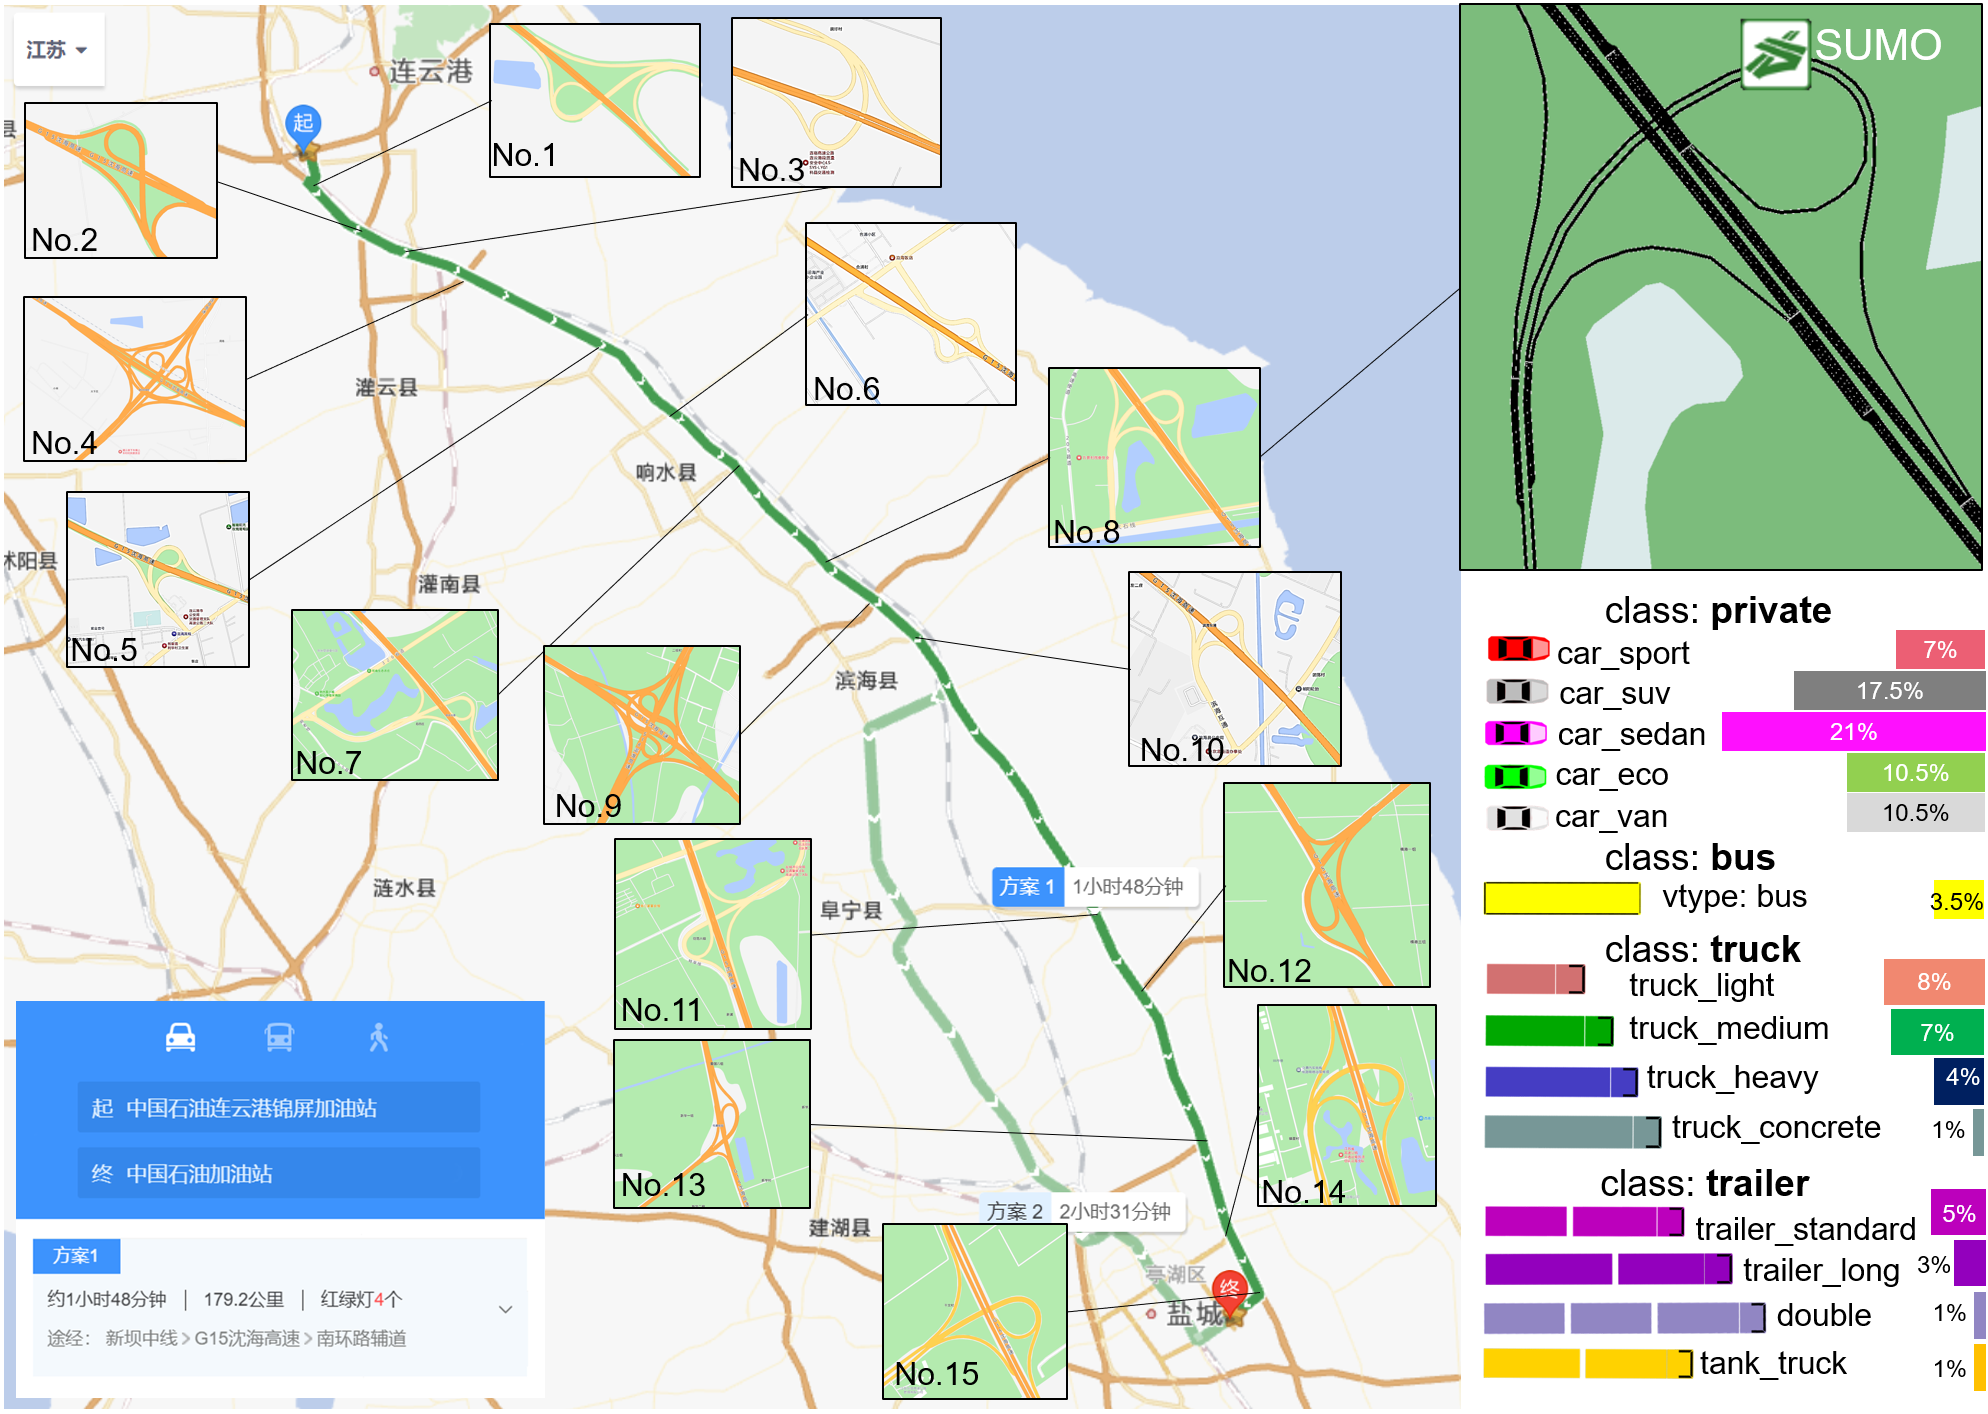
\includegraphics[width=0.95\linewidth]{fig/chap3/sim_place.png}
  \caption{G15 highway traffic simulation environment for cloud-side predictive planning.}
  \label{fig:cloud_sim_place}
\end{figure}

Graphflow was trained for a 20 s prediction horizon. Fig.~\ref{fig:graphflow_validation} reports the training loss and qualitative prediction examples. With scheduled sampling, the ego occupancy feature remains below about 1\% MSE, the risk-field feature remains below about 2\% MSE, and surrounding-vehicle occupancy remains below about 3\% MSE in the reported training process. The qualitative results show that vehicles with stable low-speed motion remain concentrated, while fast vehicles interacting with traffic diffuse into broader low-probability regions. This behavior is consistent with the objective of long-horizon risk anticipation: the model is expected to provide risk-evolution trends rather than exact deterministic trajectories at the end of a 20 s horizon.

\begin{figure}[t]
  \centering
  \subfloat[Training loss\label{fig:train_graphflow_journal}]
    {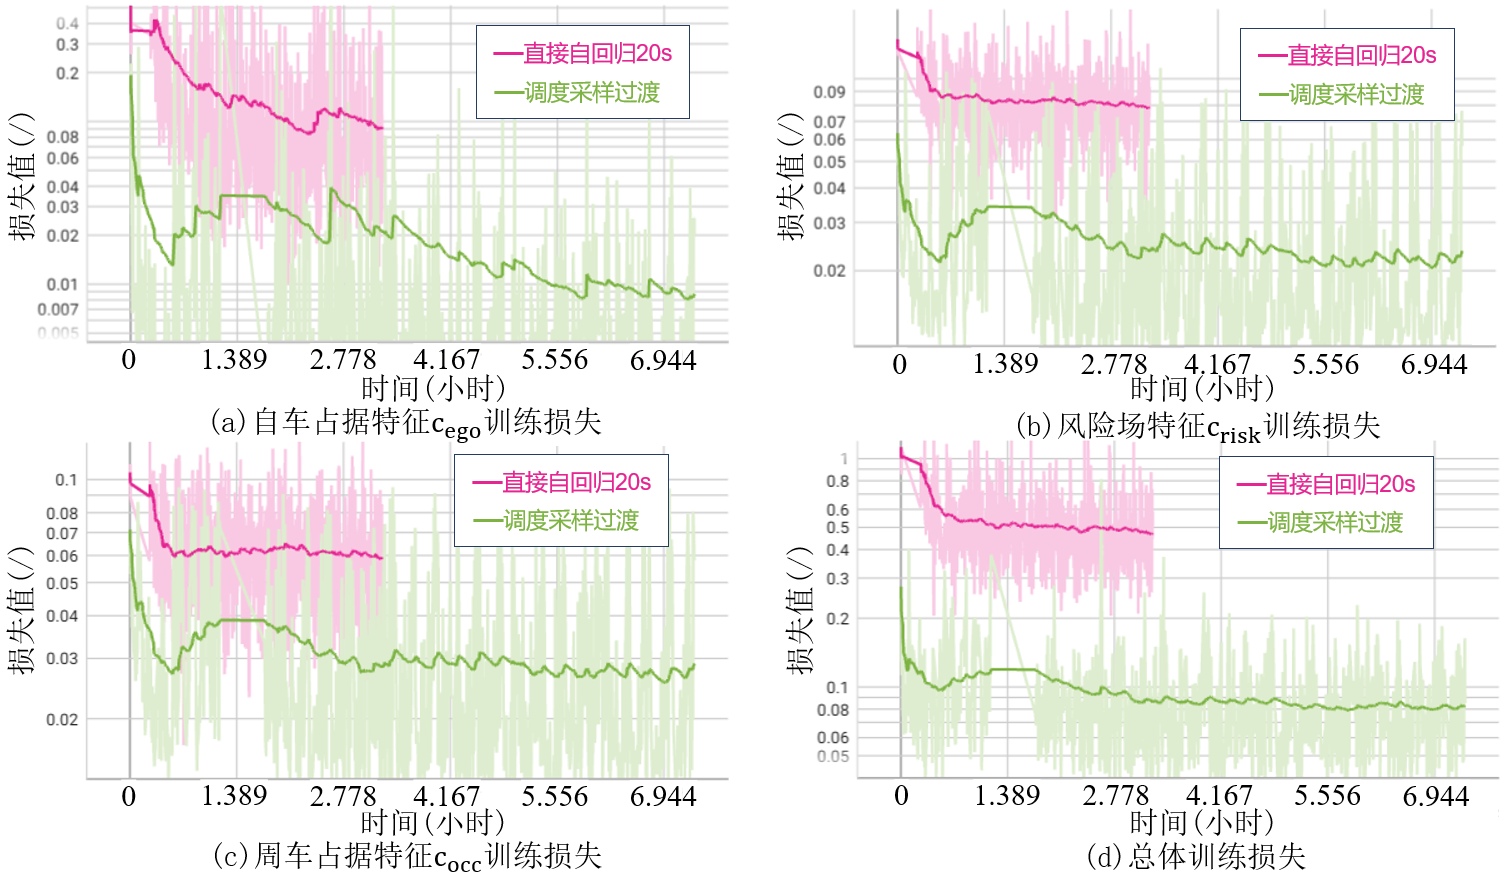
\includegraphics[width=0.92\linewidth]{fig/chap3/train_loss_graphflow.png}}\\
  \subfloat[Straight-road prediction\label{fig:risk_pred1_journal}]
    {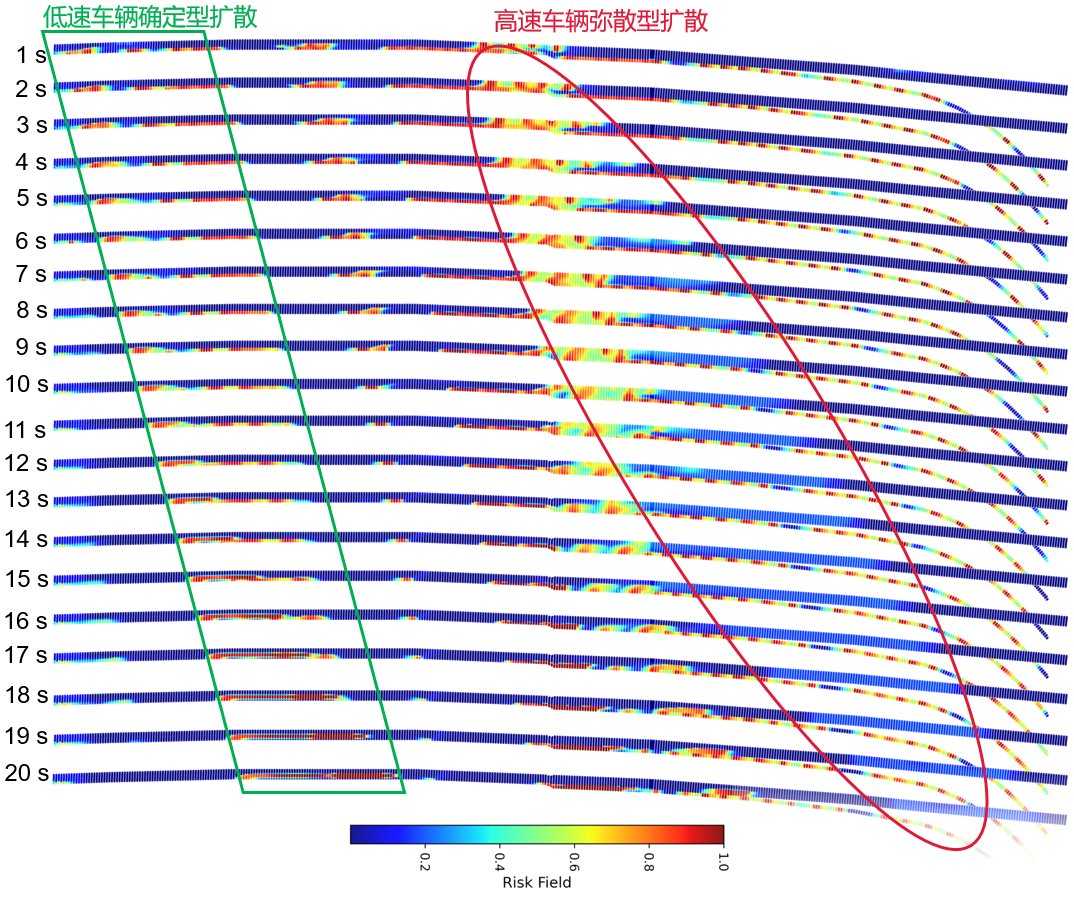
\includegraphics[width=0.92\linewidth]{fig/chap3/risk_pred1.png}}\\
  \subfloat[Interchange prediction\label{fig:risk_pred2_journal}]
    {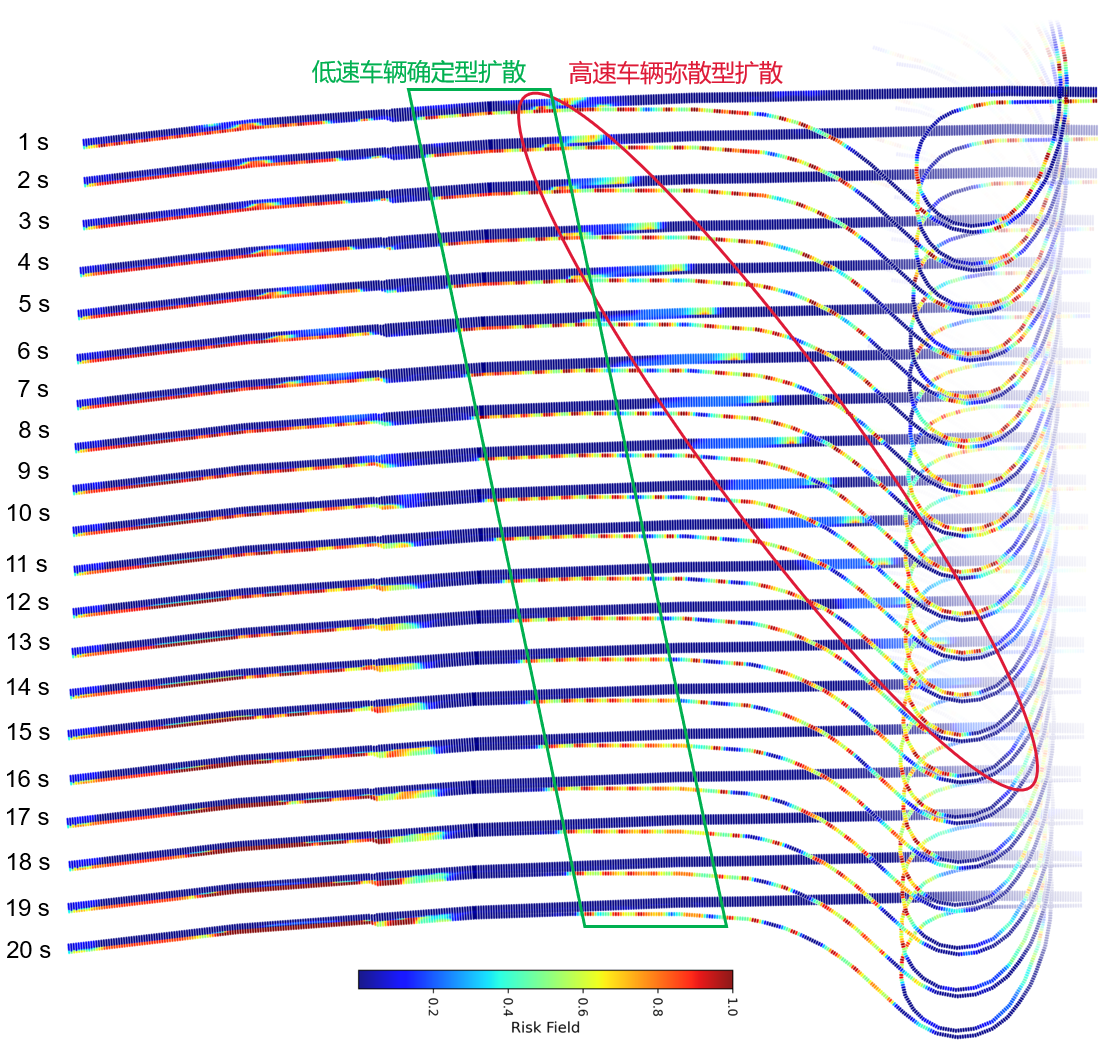
\includegraphics[width=0.92\linewidth]{fig/chap3/risk_pred2.png}}
  \caption{Graphflow training and long-horizon stochastic interaction prediction.}
  \label{fig:graphflow_validation}
\end{figure}

The cloud decision policy was trained with PPO using Graphflow as the world model and then evaluated in SUMO. Two baselines were used: a single-vehicle IDM+MOBIL policy and a decision-tree search baseline with access to the simulation model. The latter is a strong simulation-only baseline because it enumerates ego lane-change choices over a 20 s horizon, with at most three lane changes, and uses near-oracle surrounding-vehicle parameters from SUMO. The source thesis reports that the Graphflow policy achieves total scores close to the decision-tree baseline and higher than the single-vehicle baseline across the validation tasks and traffic demands. Safety improvements are most evident in the trailer-oriented modified emergency index and headway-related risk, while efficiency, comfort/economy, rule compliance, and navigation scores remain comparable to the baselines. This indicates that long-horizon prediction improves safety without forcing overly conservative driving.

\begin{figure}[t]
  \centering
  \subfloat[Total score\label{fig:total_score_journal}]
    {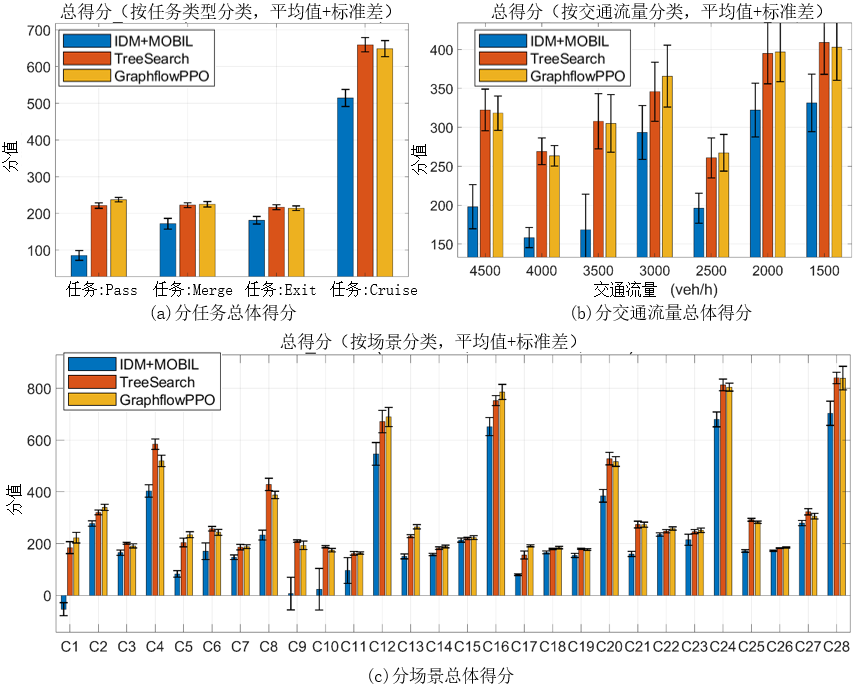
\includegraphics[width=0.92\linewidth]{fig/chap3/total_score.png}}\\
  \subfloat[Safety score\label{fig:r_safe_journal}]
    {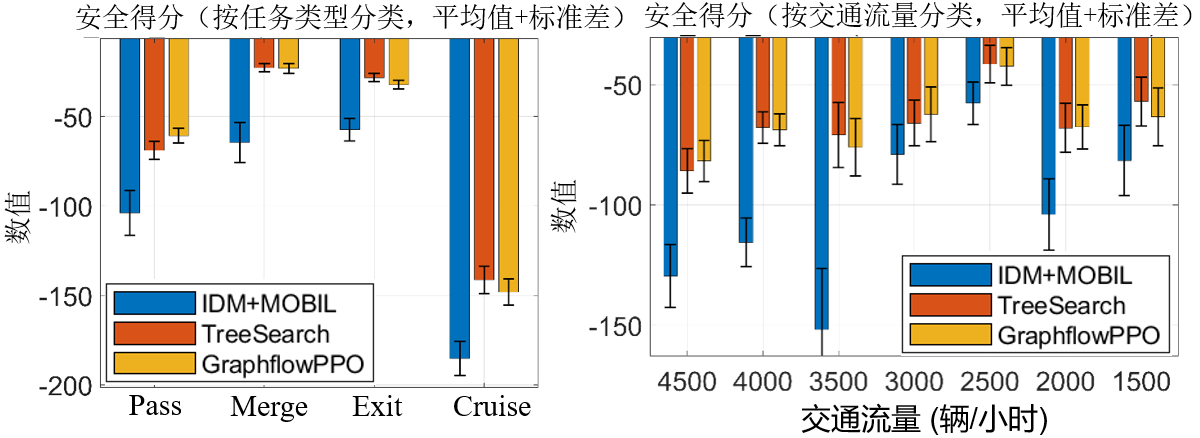
\includegraphics[width=0.92\linewidth]{fig/chap3/r_safe.png}}
  \caption{Cloud-side predictive planning performance on the validation traffic set.}
  \label{fig:cloud_scores}
\end{figure}

A representative cruising case is shown in Fig.~\ref{fig:cloud_case}. The IDM+MOBIL vehicle converges to a locally reasonable but blocked behavior. The tree-search baseline remains in the left lane for a long period, causing prolonged interaction with faster vehicles. The Graphflow policy overtakes, returns to a middle lane, and reduces parallel driving time with faster traffic while maintaining comparable travel progress.

\begin{figure}[t]
  \centering
  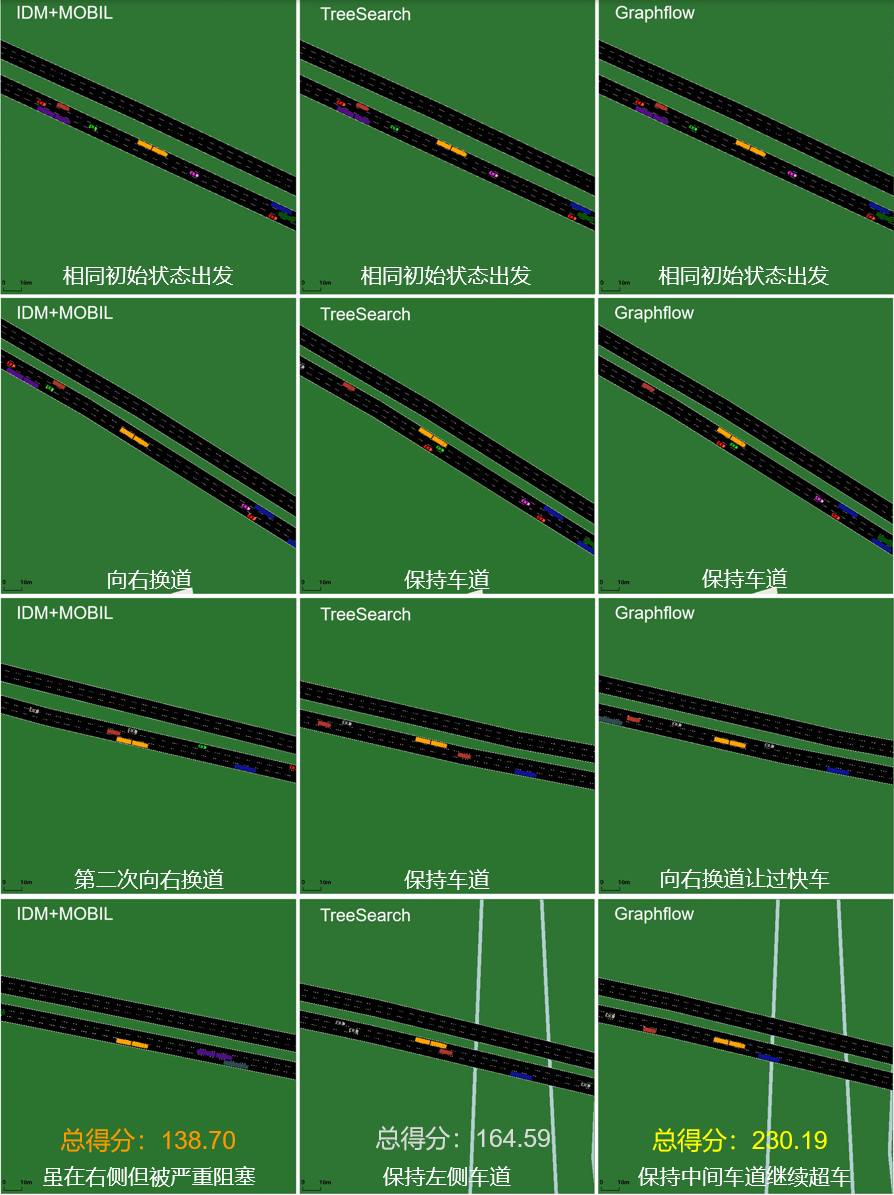
\includegraphics[width=0.95\linewidth]{fig/chap3/example_illust.png}
  \caption{Representative cloud-side planning case comparing IDM+MOBIL, decision-tree search, and Graphflow policy.}
  \label{fig:cloud_case}
\end{figure}

\subsection{Vehicle-Side Planning and Control Evaluation}

Vehicle-side planning was first evaluated in four local emergency cases derived from typical tank-truck accident mechanisms: overtaking with fast rear vehicles, left turning with an oncoming vehicle, high-speed rear approach with a parallel adjacent vehicle, and cruising beside a slow-moving queue. In these cases, the planner uses the cloud reference as the initial solution, identifies the key conflicting vehicle, constructs the most probable scenario $S_\alpha$ and the most dangerous scenario $S_\beta$, and generates a shared-prefix emergency trajectory. The qualitative results in Fig.~\ref{fig:vehicle_planning_cases} show that the planner either preserves the cloud maneuver when the dangerous mode can still be avoided or switches to braking, yielding, shoulder offset, or stopped-lane-change behaviors when the dangerous mode becomes dominant.

\begin{figure}[t]
  \centering
  \subfloat[Fast rear vehicles during overtaking\label{fig:scenario1_journal}]
    {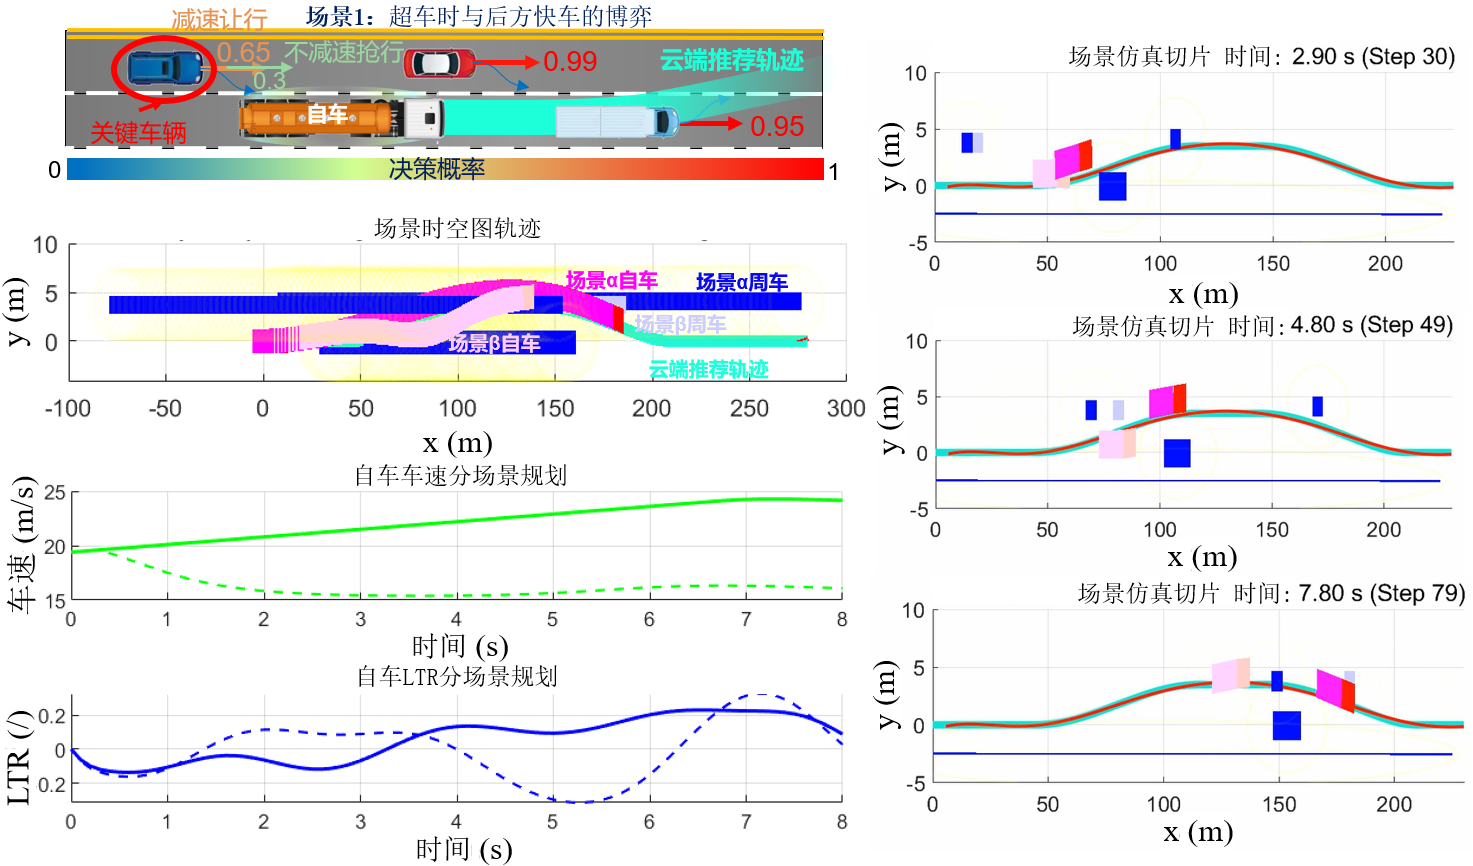
\includegraphics[width=0.48\linewidth]{fig/chap3/scenario1.png}}
  \subfloat[Oncoming vehicle during left turn\label{fig:scenario2_journal}]
    {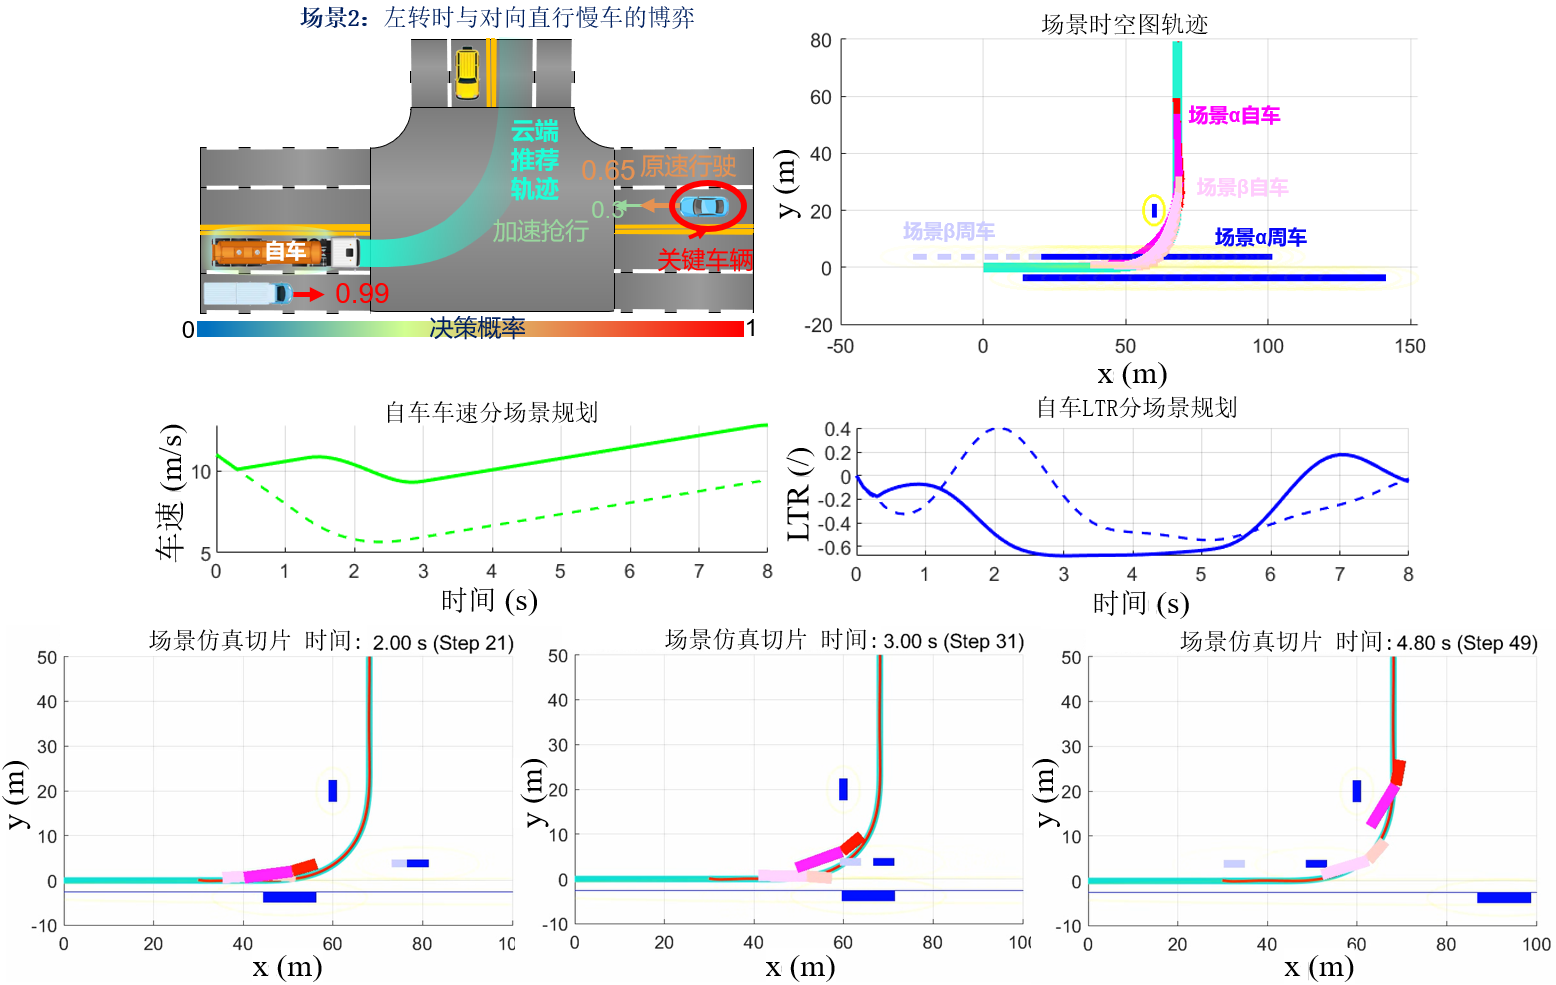
\includegraphics[width=0.48\linewidth]{fig/chap3/scenario2.png}}\\
  \subfloat[Fast rear approach with adjacent parallel vehicle\label{fig:scenario3_journal}]
    {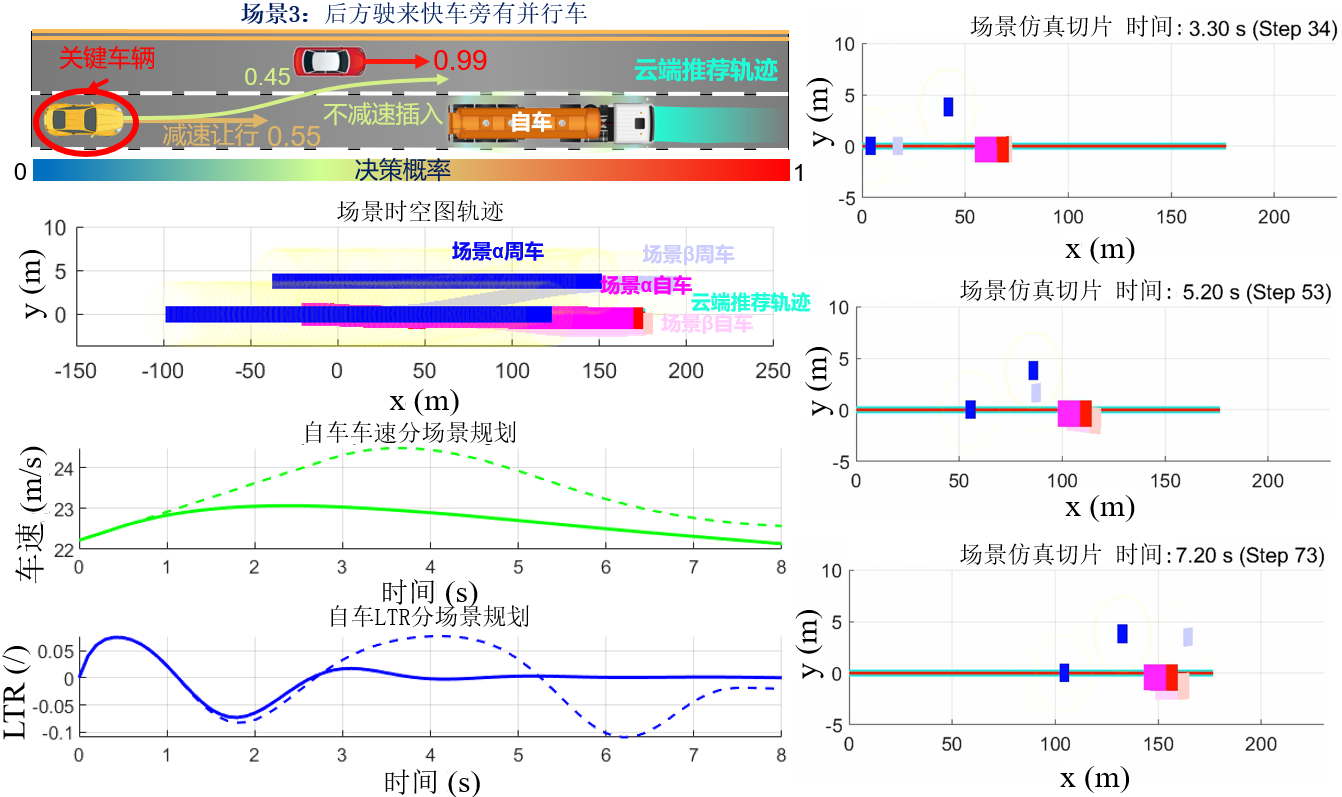
\includegraphics[width=0.48\linewidth]{fig/chap3/scenario3.png}}
  \subfloat[Slow queue beside free lane\label{fig:scenario4_journal}]
    {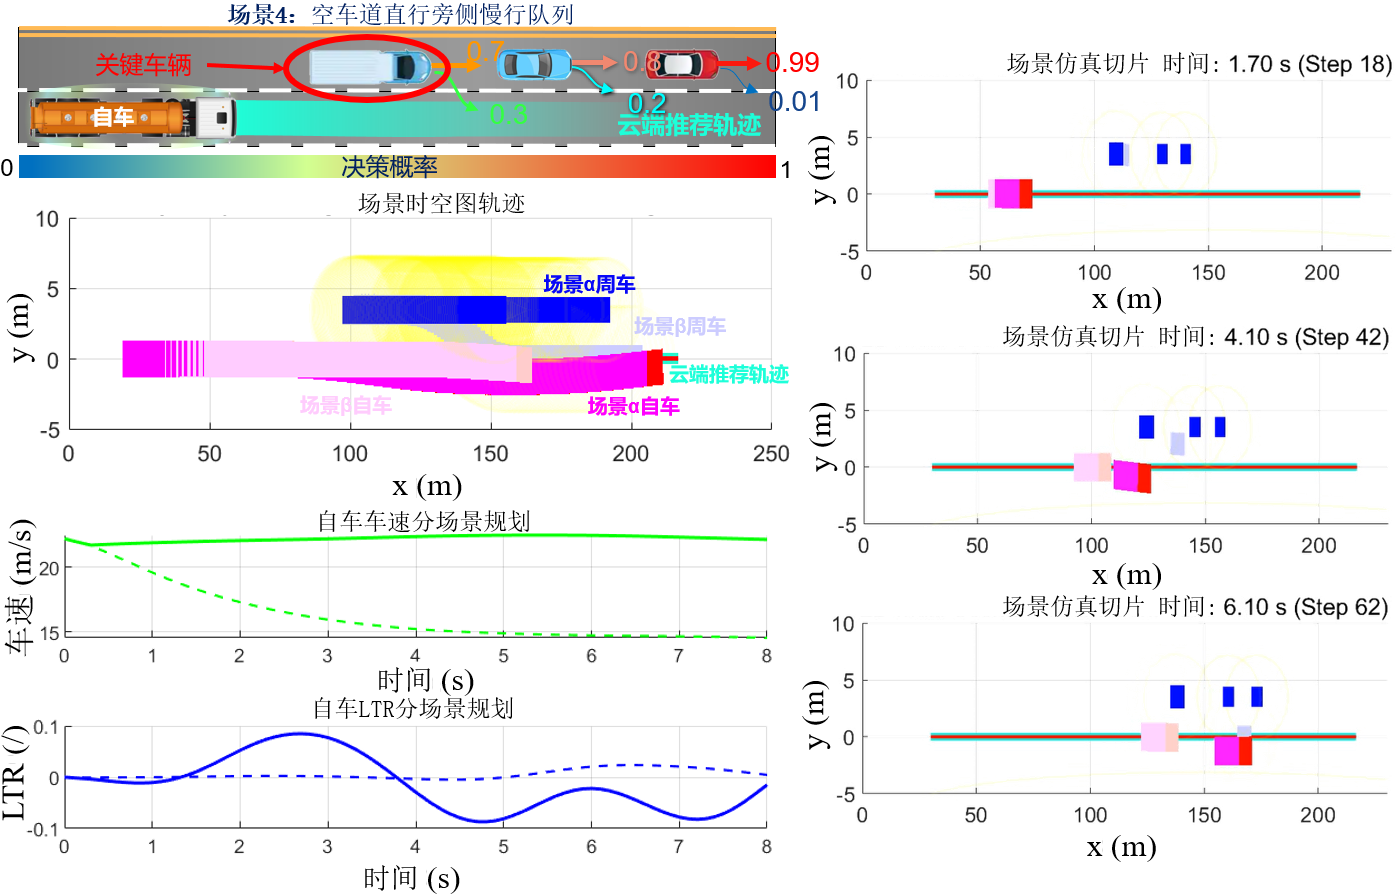
\includegraphics[width=0.48\linewidth]{fig/chap3/scenario4.png}}
  \caption{Vehicle-side emergency replanning cases.}
  \label{fig:vehicle_planning_cases}
\end{figure}

The high-frequency controller was evaluated in a TruckSim--Simulink--StarCCM+ vehicle-liquid co-simulation platform. The platform exchanges vehicle acceleration and angular motion with the CFD tank model and feeds the resulting liquid forces and moments back into the vehicle model. The CFD grid sensitivity analysis reports an average relative force/moment error below 1\% and a peak error below 4\% for the selected mesh setting. The controller frequency is 20 Hz, the co-simulation data exchange interval is 0.005 s, and the liquid filling ratio is 50\%.

\begin{figure}[t]
  \centering
  \subfloat[Co-simulation architecture\label{fig:cosim_arch_journal}]
    {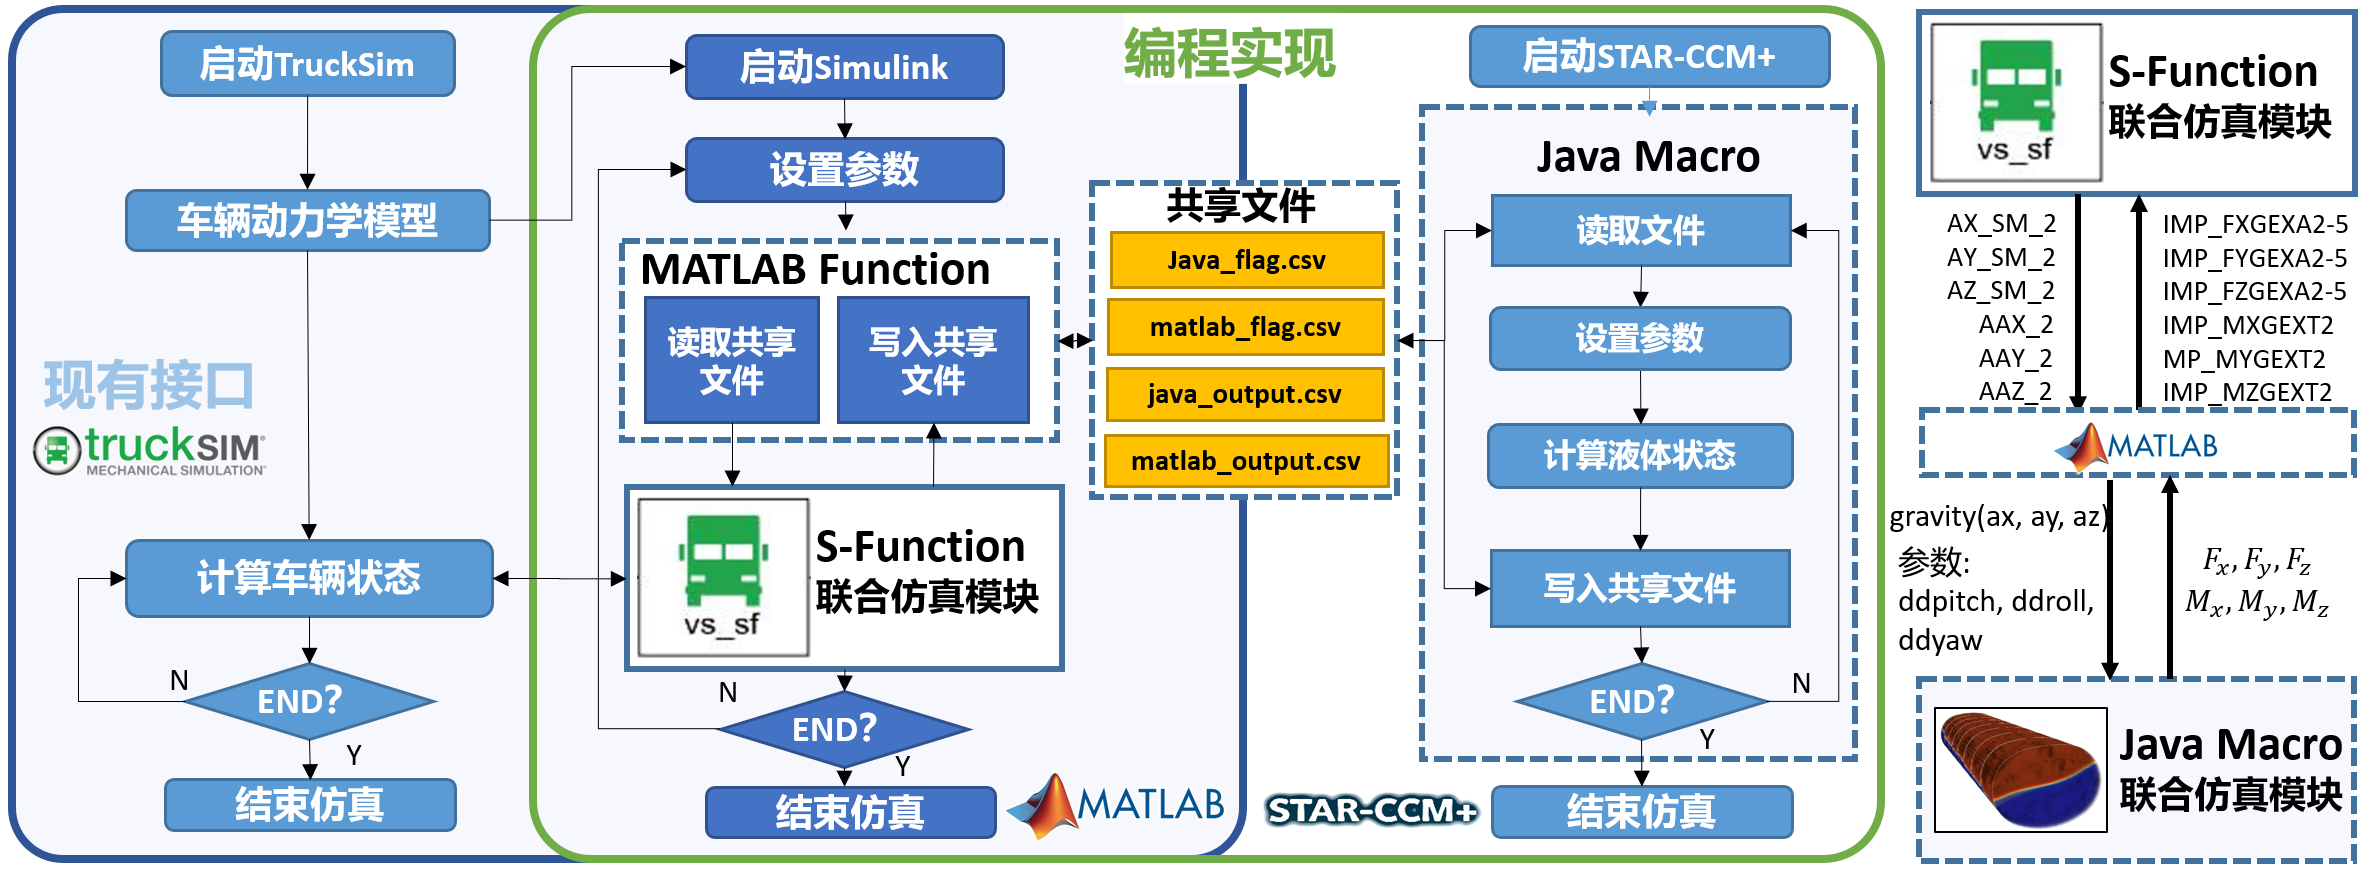
\includegraphics[width=0.94\linewidth]{fig/chap4/cosim_arch.png}}\\
  \subfloat[Grid sensitivity\label{fig:grid_sensitivity_journal}]
    {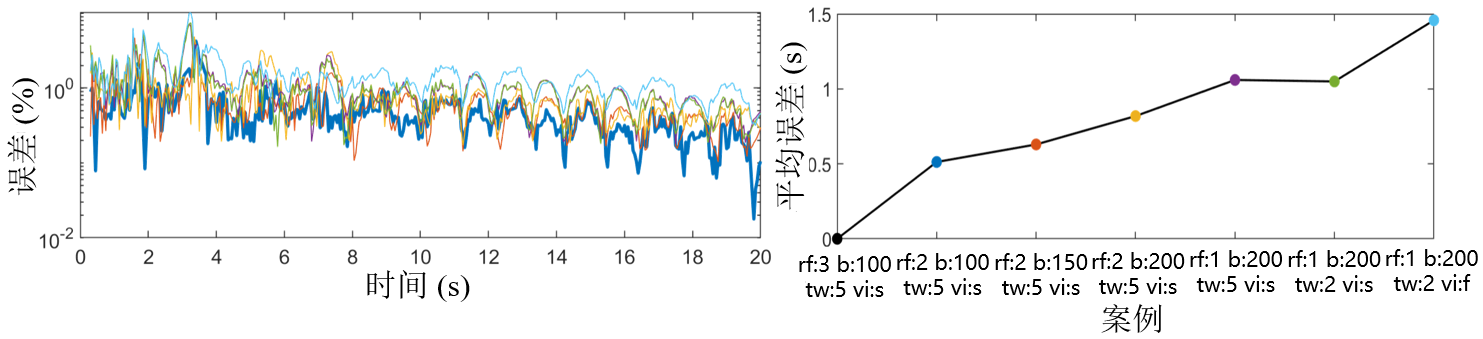
\includegraphics[width=0.94\linewidth]{fig/chap4/grid_sensitivity_res.png}}
  \caption{Vehicle-liquid co-simulation platform and CFD grid sensitivity.}
  \label{fig:cosim_validation}
\end{figure}

Four control methods were compared in the co-simulation: TruckSim preview tracking (PT), preview tracking with differential braking (PT+DB), anti-rollover tracking with steering only (ART), and the proposed anti-rollover tracking with differential braking and compensation (ART+DB). Three representative high-risk scenarios are summarized below.

In the left-turn scenario, the vehicle enters a 28.125 m left-turn radius at 35 km/h. PT rolls over at approximately 6 s. PT+DB avoids complete rollover but keeps the LTR saturated near -1 for at least 1 s. ART and ART+DB keep $\mathrm{LTR}_{eql}$ within the $\pm0.75$ soft boundary by allowing acceptable path deviation, with ART+DB producing a smaller LTR peak because differential braking assists yaw and roll stabilization.

In the SAE-J2179 single-lane-change scenario, the vehicle starts at 88 km/h and completes a 4.392 m lane change within 61 m. PT and PT+DB roll over after the lane change at around 6 s. ART sacrifices some tracking accuracy to maintain the LTR boundary. ART+DB improves tracking smoothness, uses differential braking before the risk peak, and suppresses sloshing after the maneuver.

In the short-distance double-lane-change scenario, the vehicle starts at 70 km/h, changes laterally by 3.5 m within 30 m, runs straight for 30 m, and returns within 30 m. PT already rolls over at 62 km/h in preliminary tests, confirming that the selected 70 km/h case is high risk. At 70 km/h, PT rolls over at around 6 s, PT+DB avoids complete rollover but remains near the rollover boundary for about 2.5 s, ART avoids rollover with larger tracking sacrifice, and ART+DB preserves better tracking while keeping $\mathrm{LTR}_{eql}$ within the soft boundary.

\begin{figure}[t]
  \centering
  \subfloat[Left turn\label{fig:s_corner_xu_journal}]
    {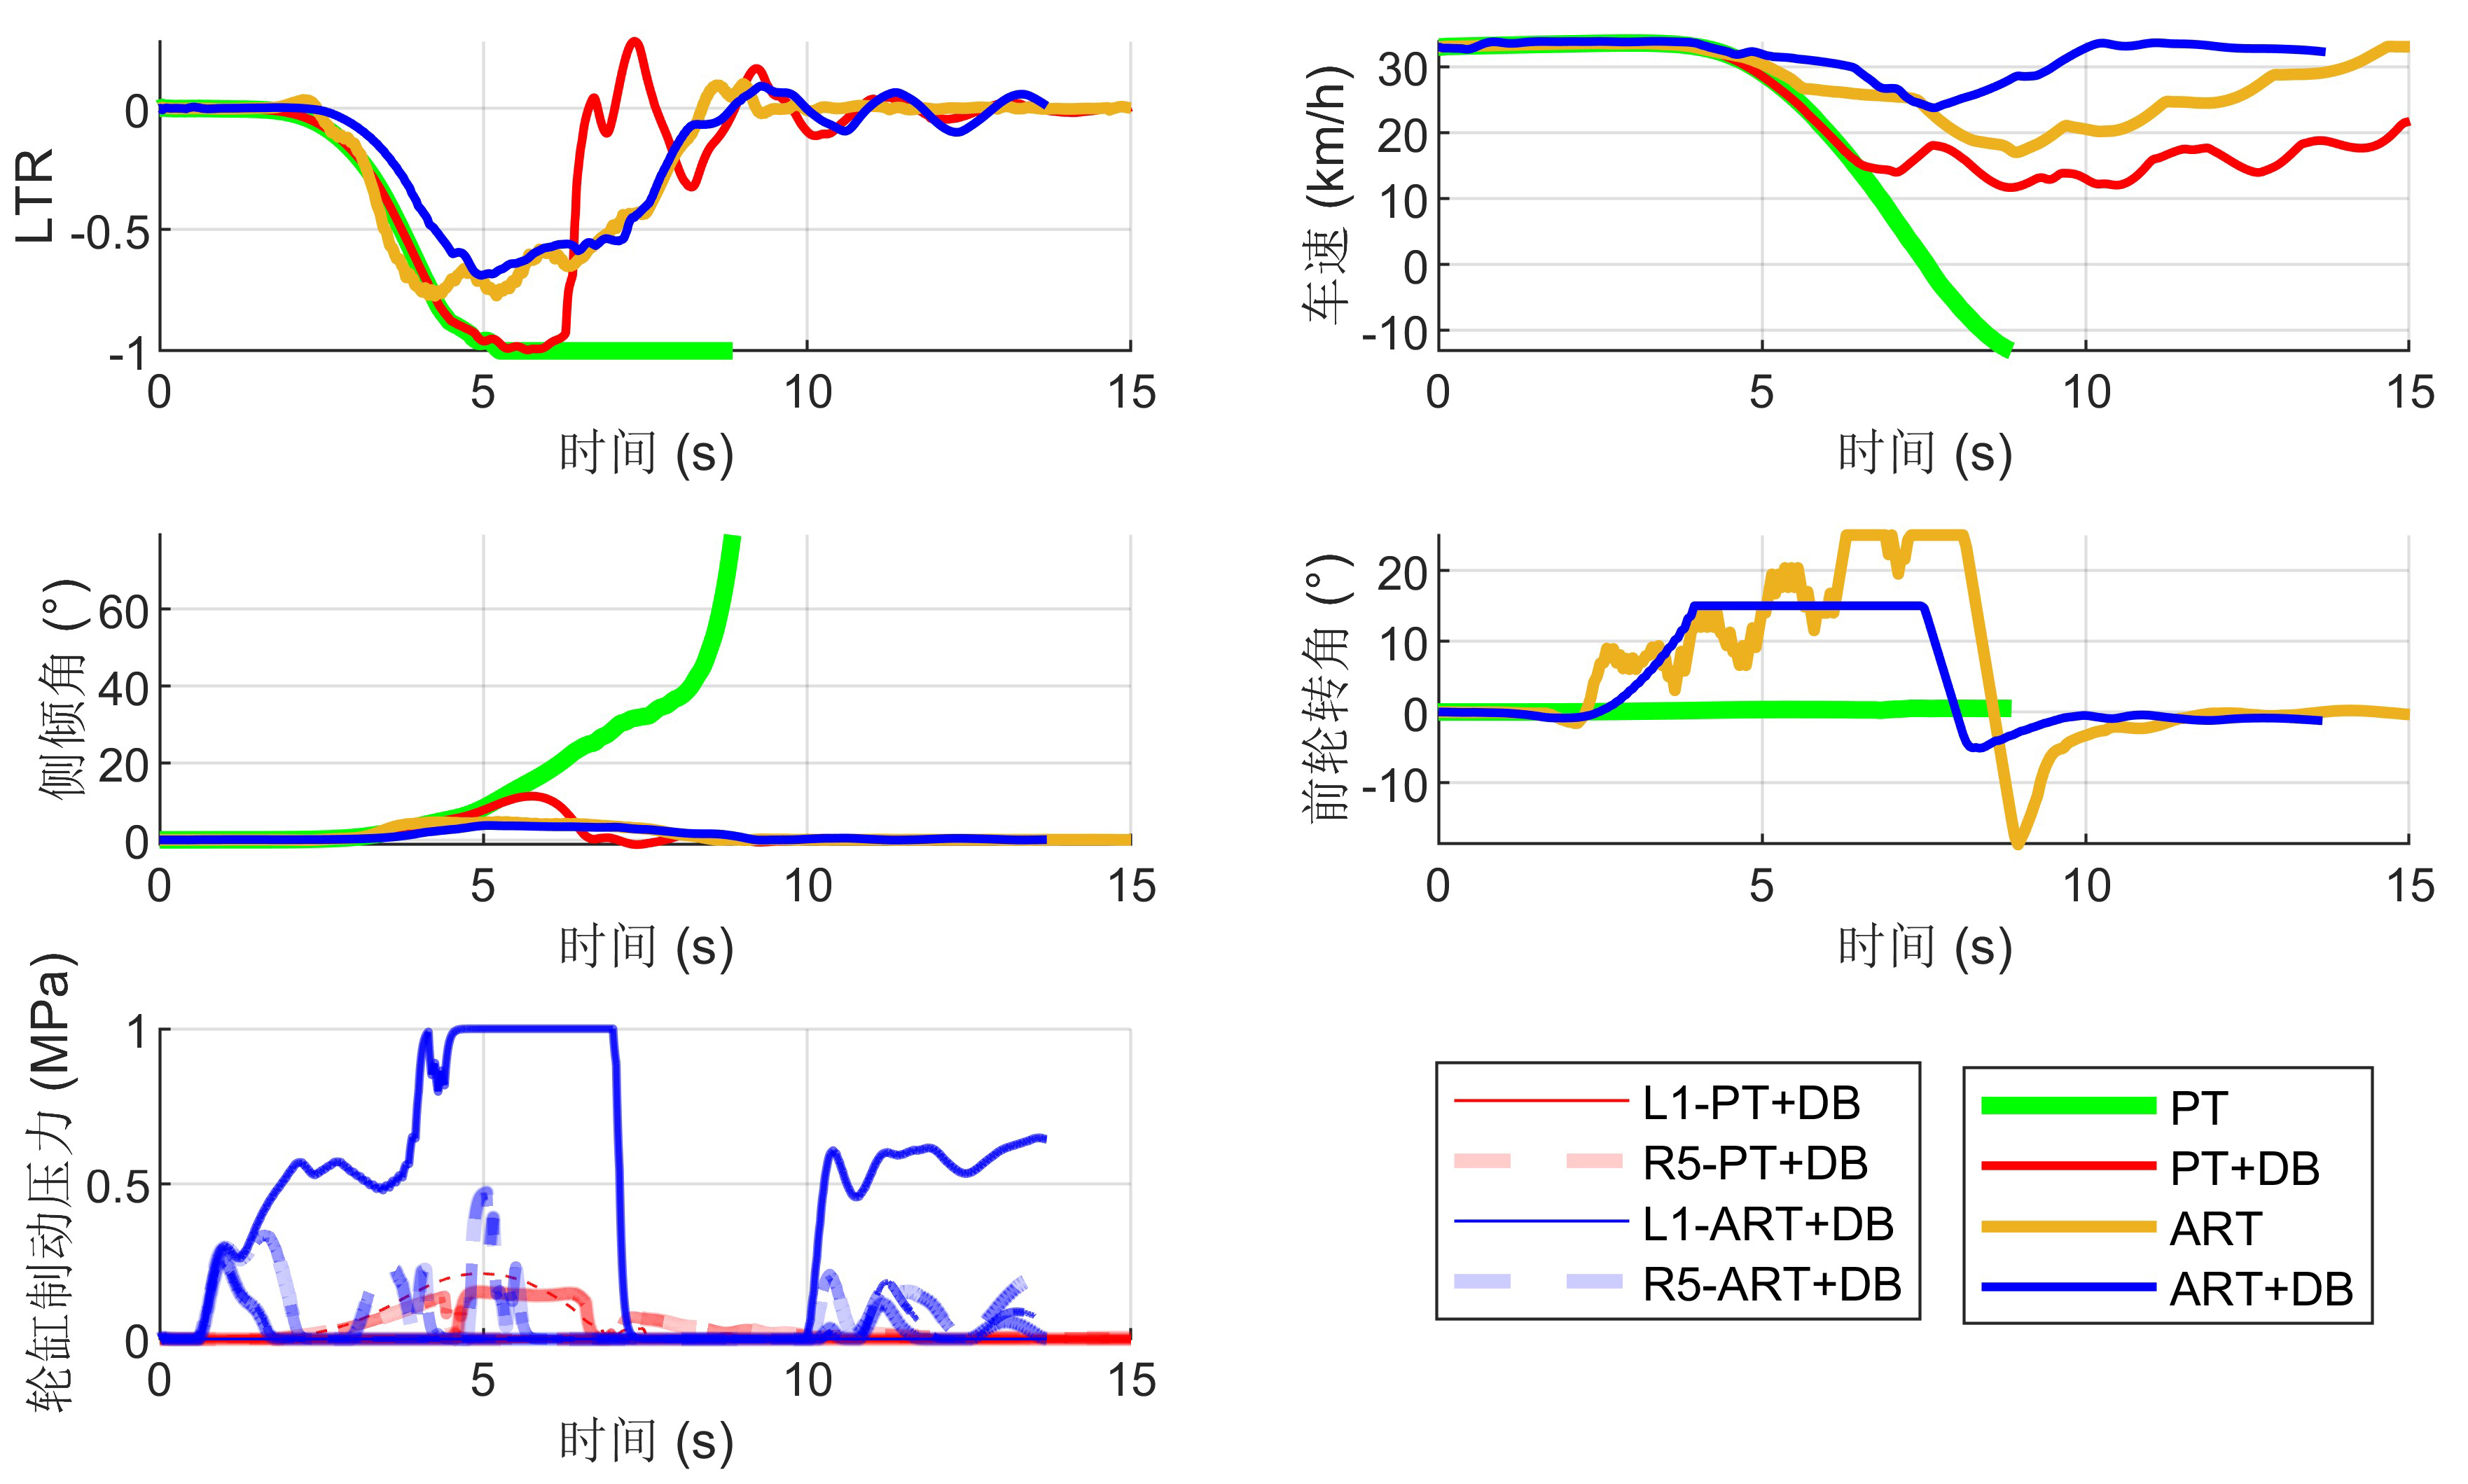
\includegraphics[width=0.95\linewidth]{fig/chap4/s_corner_xu.jpg}}\\
  \subfloat[Single lane change\label{fig:s_slc_xu_journal}]
    {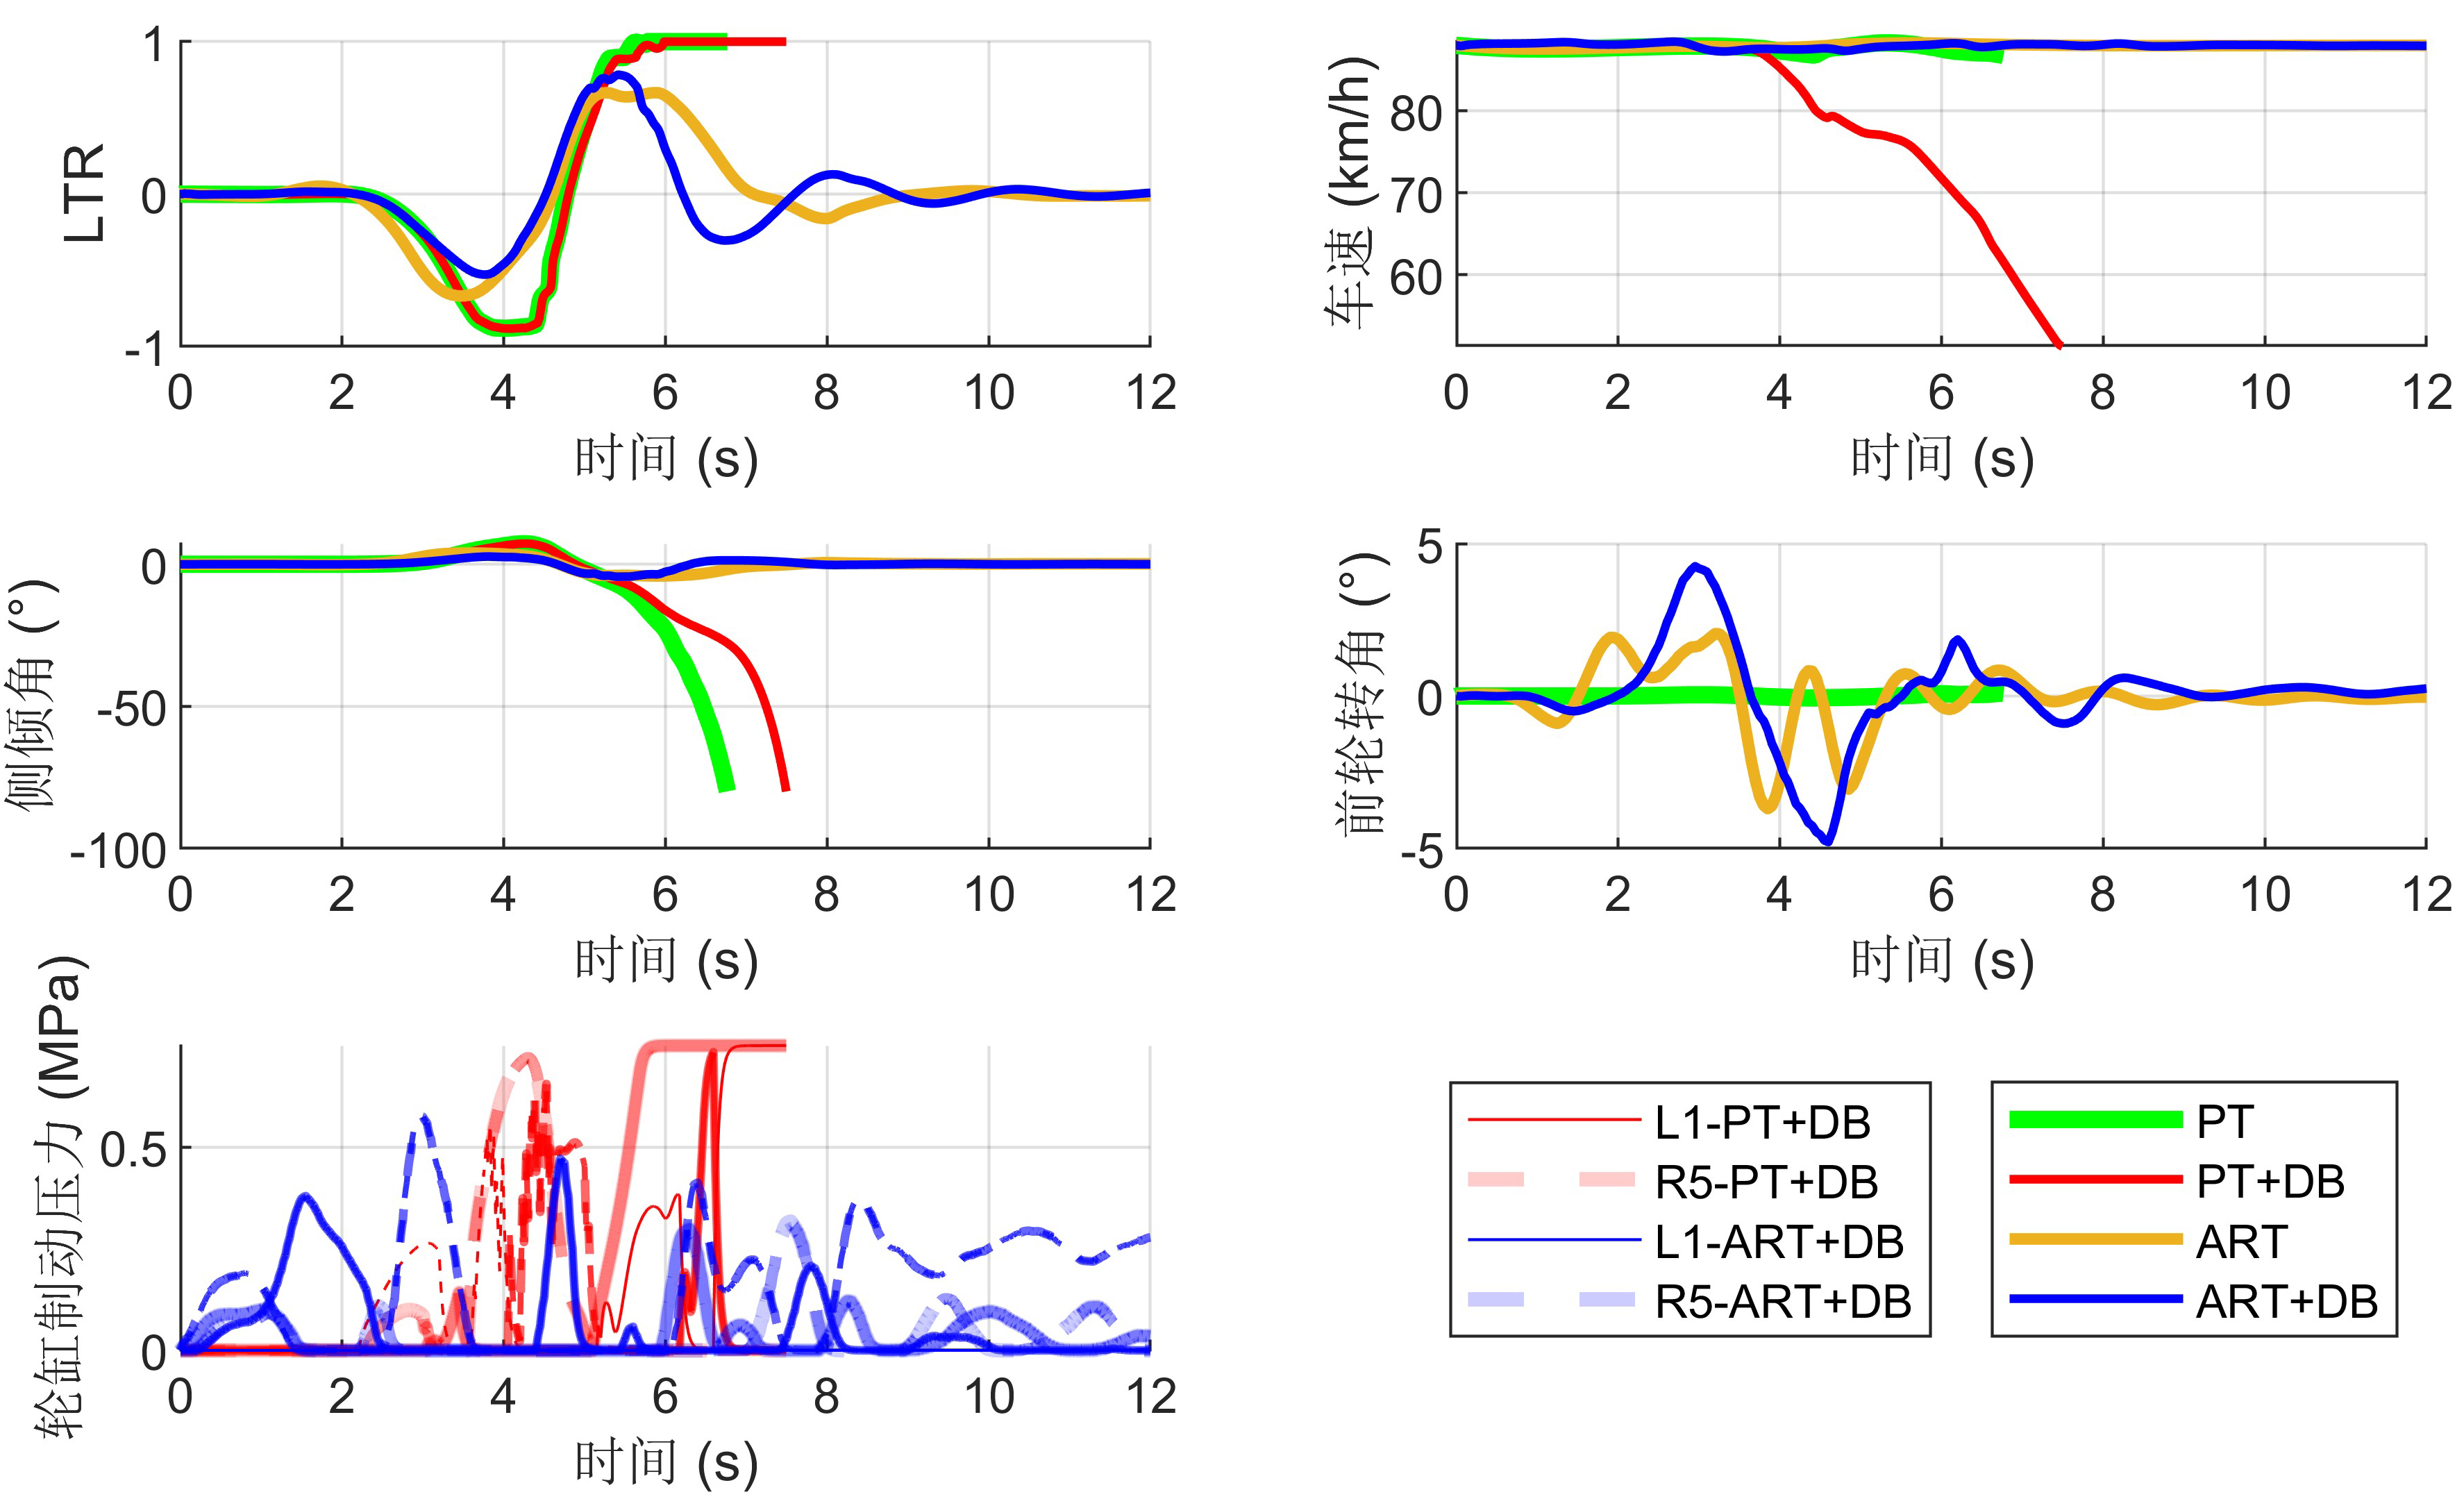
\includegraphics[width=0.95\linewidth]{fig/chap4/s_slc_xu.jpg}}\\
  \subfloat[Double lane change\label{fig:s_dlc_xu_journal}]
    {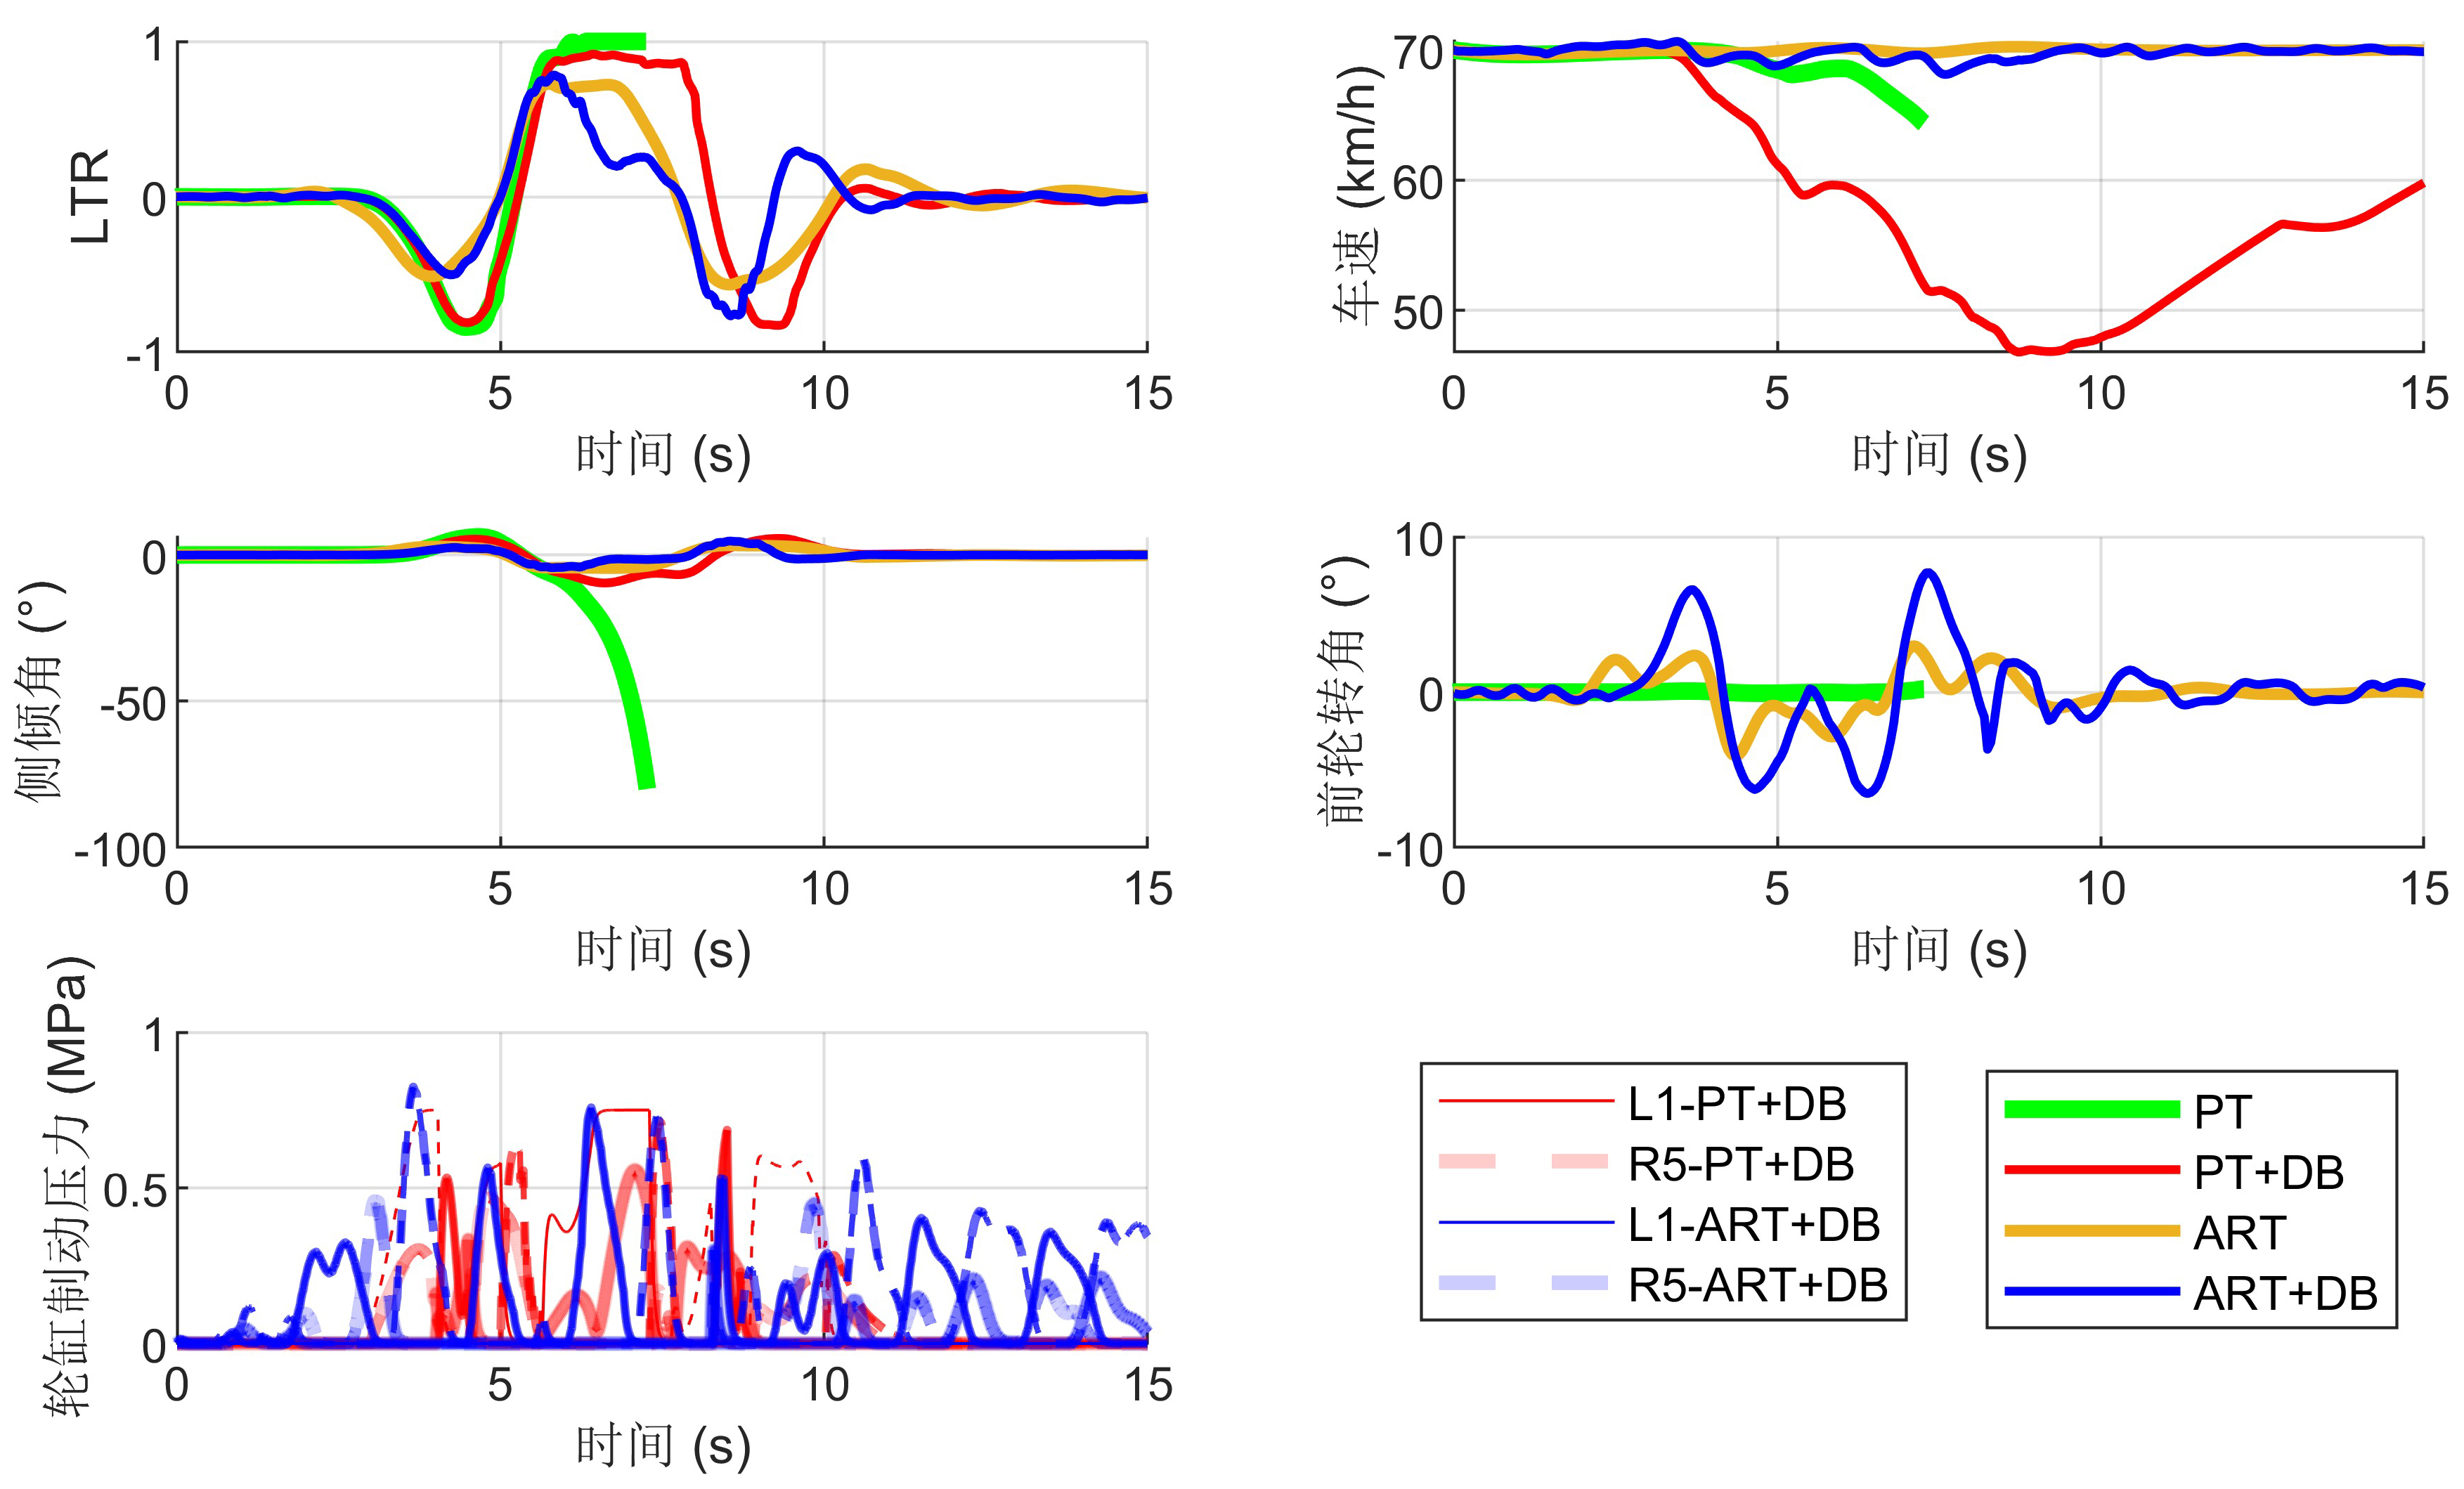
\includegraphics[width=0.95\linewidth]{fig/chap4/s_dlc_xu.jpg}}
  \caption{Vehicle-liquid co-simulation results under left-turn, SLC, and DLC scenarios.}
  \label{fig:control_cosim_results}
\end{figure}

An additional rescue test was conducted under a severe evasive maneuver. The vehicle travels at 80 km/h, the safety driver performs a sudden steering maneuver, and one-side wheel lift-off occurs at 4.7 s. PT and PT+DB continue toward rollover because they do not perform appropriate counter-steering. ART delays rollover but cannot recover without sufficient speed reduction. ART+DB combines counter-steering and strong differential braking, exits the half-rollover state, and returns toward the reference trajectory. This test indicates that the proposed controller extends the recoverable domain beyond ordinary LTR-constrained tracking cases.

\subsection{Scaled Tank-Truck Experimental Validation}

A 1:14 scaled semi-trailer tank-truck platform was built for experimental validation. The model has a total length of 1250 mm after tank installation, a width of 200 mm, a height of 350 mm, a mass of 42 kg, and a maximum speed of about 3 m/s. The platform includes IMU/GNSS units, wheel encoders, perception sensors, a Jetson Orin NX controller, and an acrylic liquid tank with anti-surge plates. Similarity analysis was used to relate the scaled test to prototype lateral acceleration and liquid-sloshing time scale. For free-surface sloshing, the Froude number and the sloshing-period relation were used to design the double-lane-change test trajectory.

\begin{figure}[t]
  \centering
  \subfloat[Hardware platform\label{fig:hardware_journal}]
    {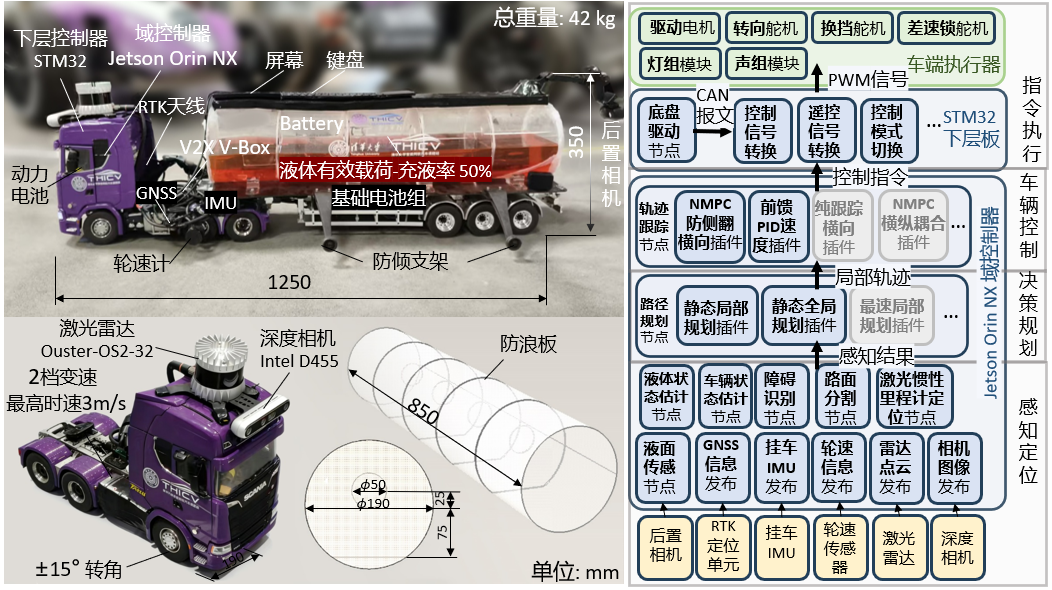
\includegraphics[width=0.95\linewidth]{fig/chap4/hardware.png}}\\
  \subfloat[Similarity and reference design\label{fig:exp_ref_pic_journal}]
    {\includegraphics[width=0.95\linewidth]{fig/chap4/exp_ref_traj.jpg}}
  \caption{Scaled tank-truck experimental platform and reference trajectory design.}
  \label{fig:scaled_platform}
\end{figure}

The experiment compares pure tracking and anti-rollover control. The controller runs at 20 Hz with prediction horizon $N_p=15$, control horizon $N_c=5$, and constrained horizon $N_r=5$. In low-speed slalom, both methods maintain small tracking errors. In the high-speed short-distance double-lane-change test, both vehicles maintain approximately 2.5 m/s, but the pure-tracking case produces severe sloshing and touches the anti-rollover support during 3--3.5 s and 4--4.5 s of the maneuver. This support contact corresponds to rollover in a full-scale unprotected vehicle.

The anti-rollover controller delays the return to the original lane and keeps the LTR inside the soft boundary. The trailer roll angle remains within about $\pm5\degree$, and the liquid free-surface angle remains approximately within $[-15\degree,15\degree]$. In contrast, the pure-tracking method reaches about 6--7 degrees trailer roll during the two lane-change peaks, the LTR reaches 1 around 3 s and 4.5 s, and the liquid angle exceeds 20 degrees multiple times. The maximum roll-angle reduction of the anti-rollover controller is about 42\%. The average solver time is 15.4 ms, and the peak solver time is below 25 ms.

\begin{figure}[t]
  \centering
  \subfloat[Experiment photographs\label{fig:cond_pic_journal}]
    {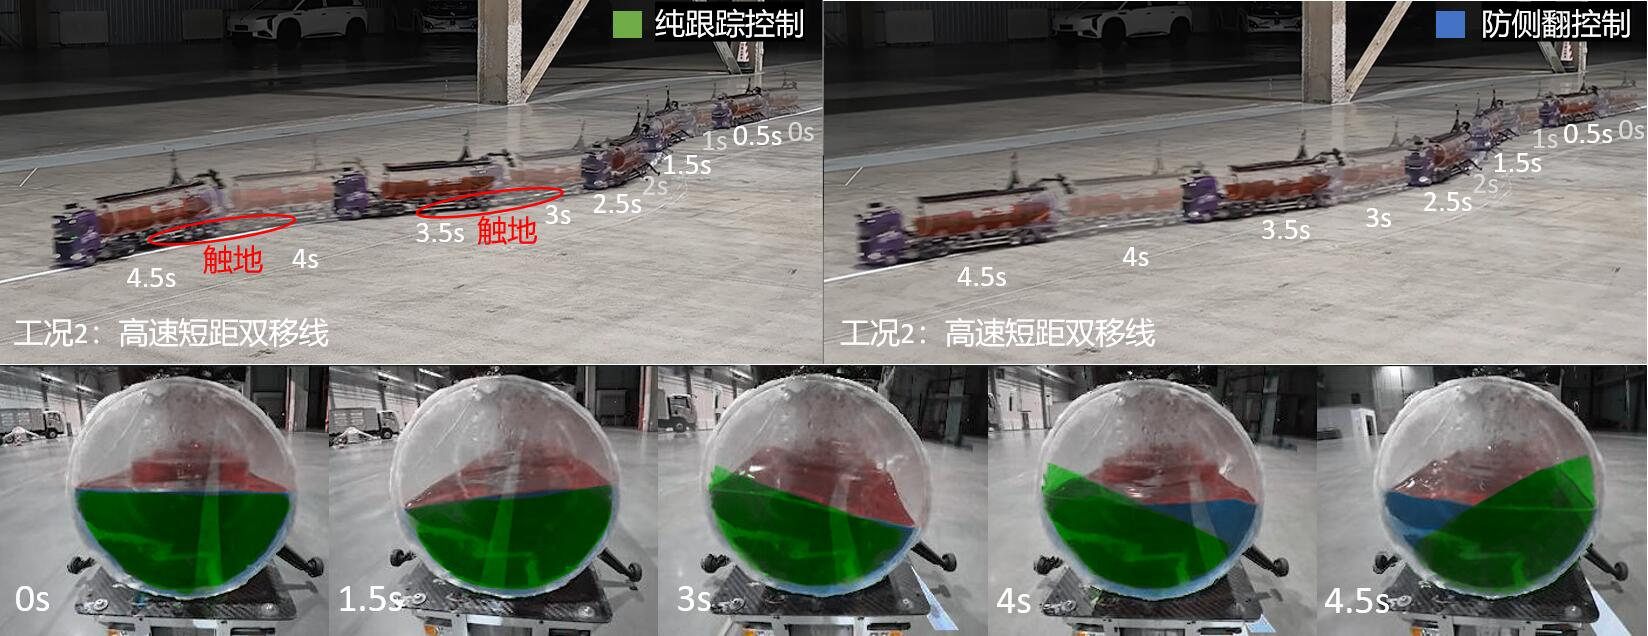
\includegraphics[width=0.95\linewidth]{fig/chap4/cond2_pic.jpg}}\\
  \subfloat[Trajectory tracking\label{fig:exp_traj_journal}]
    {\includegraphics[width=0.95\linewidth]{fig/chap4/exp_traj.jpg}}\\
  \subfloat[Vehicle states\label{fig:exp_x_journal}]
    {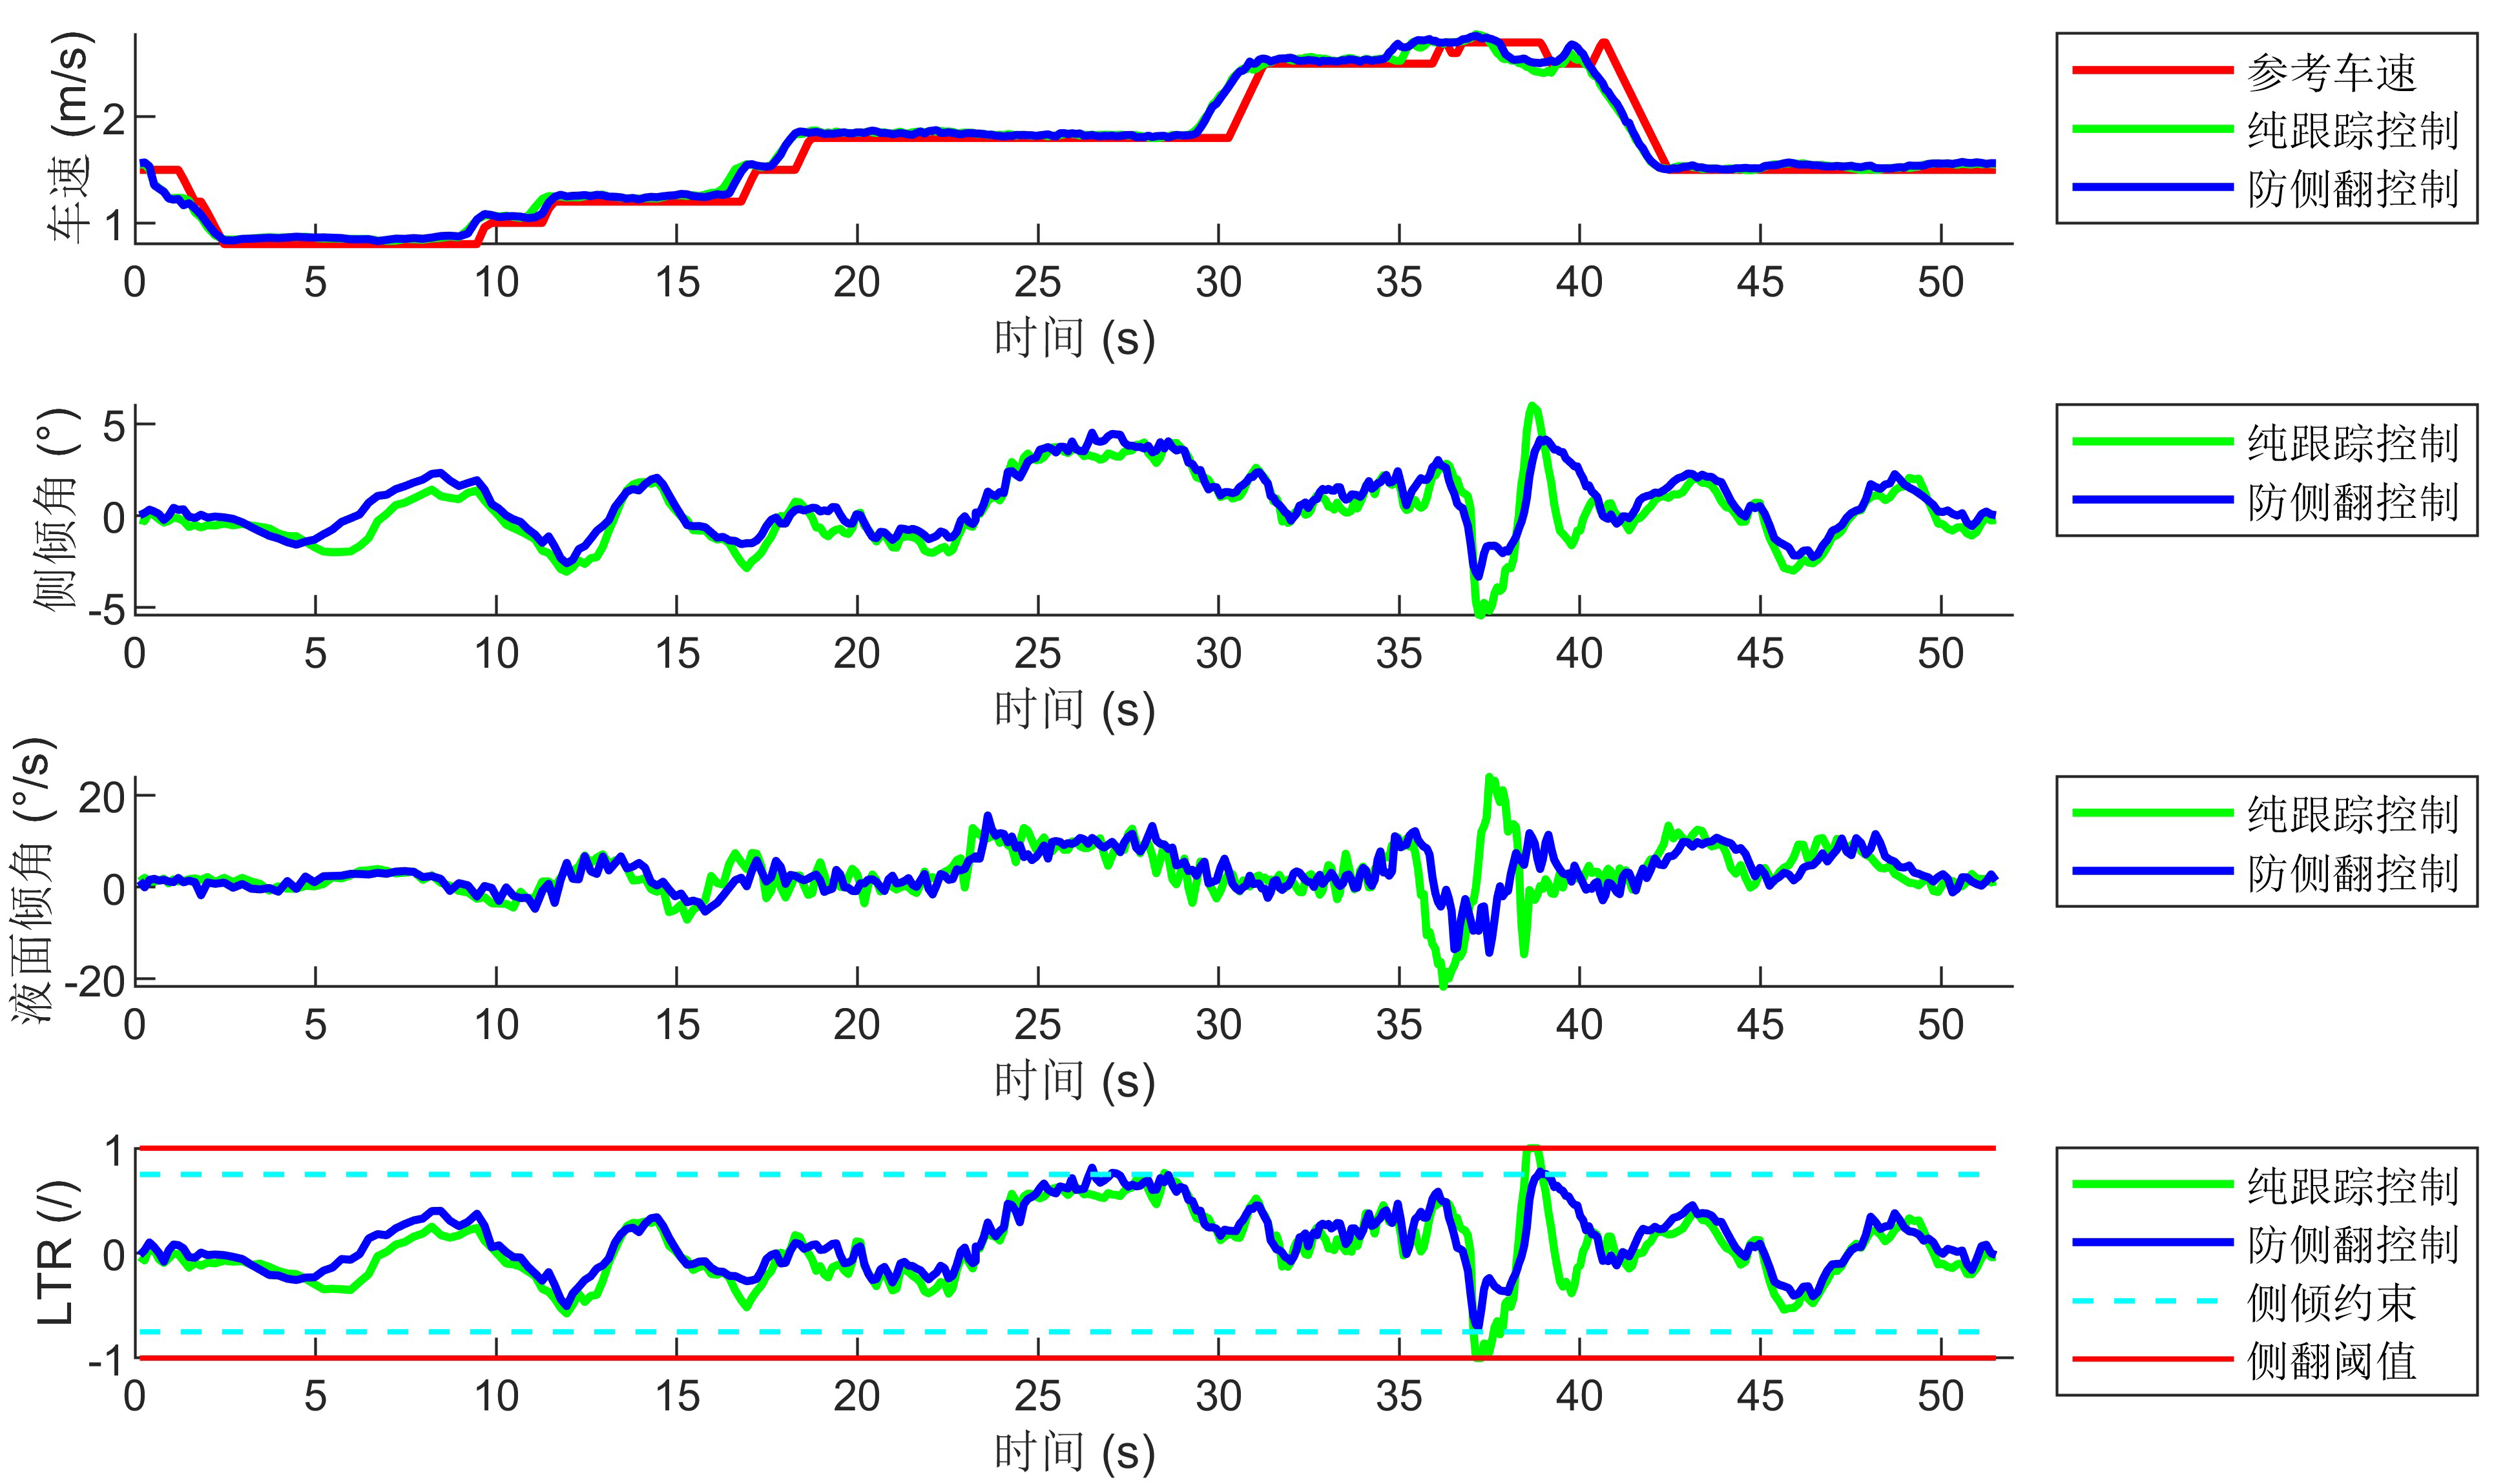
\includegraphics[width=0.95\linewidth]{fig/chap4/exp_x.jpg}}\\
  \subfloat[Control and solver time\label{fig:slack_iter_journal}]
    {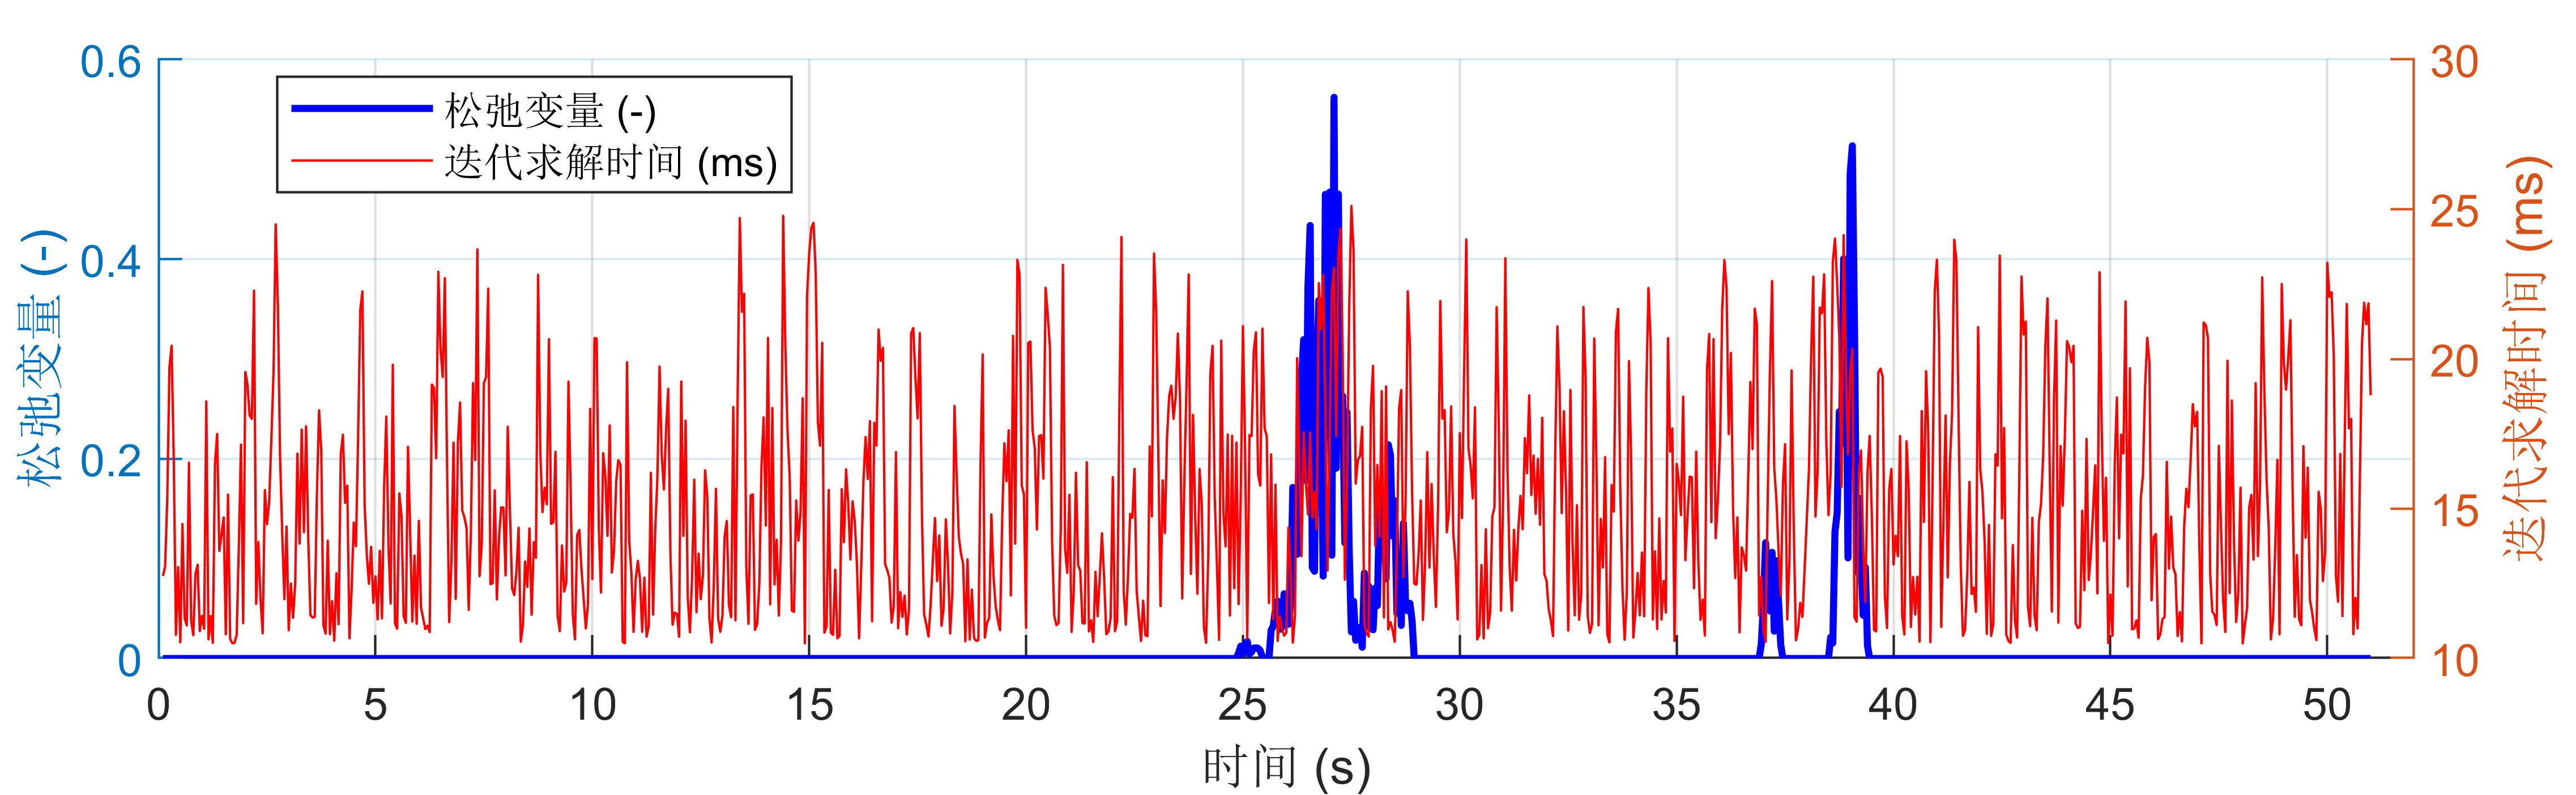
\includegraphics[width=0.95\linewidth]{fig/chap4/slack_iter.jpg}}
  \caption{Scaled model-truck experimental validation.}
  \label{fig:model_experiment_results}
\end{figure}

\subsection{Ablation and Real-Time Analysis}

The available validation supports the role of each major layer. Removing long-horizon prediction reduces the system to the single-vehicle IDM+MOBIL baseline, which is consistently less safe in the traffic validation set. Removing rollover-aware execution reduces the system to PT or PT+DB, which fails or approaches the rollover boundary in the high-risk co-simulation cases. Removing the coupled steering-braking MPC compensation reduces the system to ART, which can prevent rollover but sacrifices more tracking performance and has less recovery capability in the rescue case. Table~\ref{tab:ablation_plan} summarizes the ablation evidence currently available from the thesis.

\begin{table*}[t]
  \centering
  \caption{Ablation Evidence Available in the Current Draft}
  \label{tab:ablation_plan}
  \begin{tabularx}{0.96\textwidth}{p{0.24\textwidth}p{0.35\textwidth}X}
    \toprule
    Removed module & Available comparison & Main observation \\
    \midrule
    Cloud-side prediction and RL decision & IDM+MOBIL vs. Graphflow policy in 280 validation runs & Predictive planning improves safety-related scores while keeping efficiency comparable. \\
    Rollover-aware reference and control & PT vs. ART/ART+DB in left-turn, SLC, and DLC co-simulation & Pure tracking rolls over in multiple high-risk scenarios. \\
    Differential braking and compensation in MPC & ART vs. ART+DB in co-simulation & ART+DB improves tracking and recovery while keeping LTR within the soft boundary. \\
    Anti-rollover MPC in scaled tests & Pure tracking vs. anti-rollover control & Anti-rollover control reduces maximum roll angle by 42\% and avoids support contact. \\
    \bottomrule
  \end{tabularx}
\end{table*}
% TODO: Complete a numerical ablation table after extracting uniform metrics from the simulation logs: maximum tracking error, maximum LTR, maximum roll angle, sloshing amplitude, collision/conflict rate, and solver time for each module combination.

Real-time feasibility is supported at two levels. On the cloud side, Graphflow and PPO are trained offline; online inference provides low-frequency predictive guidance. The reported training times are 6.9 h for Graphflow and 8.3 h for the PPO decision model on a single RTX 5070 Laptop GPU. On the vehicle side, the scaled platform demonstrates 20 Hz MPC execution with an average solution time below the 50 ms control period. Full cloud-edge deployment tests with communication delay and packet loss remain future work.
